\subsection{\textcolor{Blu}{ BUCT } }
\vspace{5mm}
\begin{center}
\large{
  \textbf{ DeliGHtFAL: Delivering GABA and 5HTP through Fatty Acid Lowering }\\

  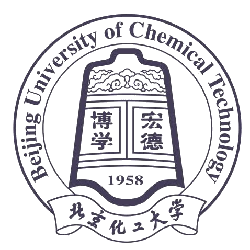
\includegraphics[width=4cm,height=4cm]{BUCT}
}
\end{center}
\textbf{\\Team Leader}

  陈青黎

  林羿妙

  莫淇茜*


\textbf{\\Contact}

  buct\_igem@163.com


\textbf{\\A Therapeutics Project\\}\begin{spacing}{1.5}

Humans have been plagued by obesity and anxiety for a long period of time. Studies have shown that obesity can aggravate anxiety while depression and anxiety also fuel obesity, namely the depression-obesity circle. In order to break this circle and alleviate people's body shame and anxiety, we used \textit{E. coli} Nissle 1917 as a chassis with enhanced capacity of β-oxidation of fatty acid thereby increasing fatty acids consumption from diets to facilitate weight loss. Meanwhile, GABA and 5-HTP with anxiety-relieving effects were synthesized from the catabolic products of fatty acids and glycerol in our engineered bacteria. To sum up, this project aims to ameliorate obesity and anxiety simultaneously by converting fatty acids, which causes body shame, to GABA and 5-HTP, ultimately breaking the depression-obesity circle.

长期以来,人们备受肥胖和焦虑的困扰。研究表明,肥胖和焦虑之间存在着双向影响,即“depression-obesity circle”。为缓解这种循环带来的“body shame”以及焦虑等烦恼,我们利用 \textit{E. coli} Nissle 1917 底盘,通过加强它对人们日常饮食中的脂肪酸的β氧化反应帮助人们减肥。同时采用合成生物学思想,利用工程菌分解脂肪的前体物质合成具有缓解焦虑效果的GABA和5-HTP。\end{spacing}
\\

\url{https://2021.igem.org/Team:BUCT }\\
\url{https://igem.org/Team.cgi?id=3875 }\\
\url{http://parts.igem.org/wiki/index.php?title=Part:BBa_K3875000 }\\
\url{https://video.igem.org/w/9vDXKPTXmELUsiQX2dtmmA }\\

\vfill{}









Team of BUCT will present between    2021/8/28 8:30-10:00     using 腾讯会议 404 469 7665.
\newpage


\subsection{\textcolor{Blu}{ NEU\_CHINA } }
\vspace{5mm}
\begin{center}
\large{
  \textbf{ Environmental multivirus detection based on PmrCAB and LuxI/LuxR quorum sensing system }\\

  
\includegraphics[width=4cm,height=4cm]{NEU_CHINA}
}
\end{center}
\textbf{\\Team Leader}

  吴自涵


\textbf{\\Contact}

  1172553993@qq.com


\textbf{\\A Diagnostics Project\\}\begin{spacing}{1.5}

Over the years, humans have suffered from coronavirus several times, and today we still troubled by SARS-CoV-2. It's unknown whether we will be affected by the coronavirus in the future. Detection of environmental coronavirus would be a critical step for cutting off the source and route of its infection. Therefore, it is necessary to design a multivirus detector to help solve epidemic caused by coronavirus. In this study, we developed an environmental multivirus detection device based on engineered \textit{E. coli} to capture coronavirus, such as SARS-CoV-2, MERS-CoV and HCoV-229E, to spark fluorescence reporter gene. The PmrCAB system derived from Salmonella was recombined onto the surface of \textit{E. coli}, and the Fe(III) recognition site of PmrB was replaced with the receptor of targeted coronavirus. Therefore, the bacteria can capture coronavirus via binding to their receptors and transport signaling to the downstream components. LuxI/LuxR quorum sensing system from \textit{E. coli} and Hrp amplifier from \textit{Pseudomonas syringae} were used to enhance the sensitivity and output signal. In addition, we also develop an improved air sampler to enrich nanoparticle in air onto engineered \textit{E. coli}. The implementation of the environmental multivirus detection would be helpful for establish a preventive system in public place, such as hospital and super market.\end{spacing}
\\

\url{https://2021.igem.org/Team:NEU\_CHINA }\\
\url{https://igem.org/Team.cgi?id=3896 }\\
\url{http://parts.igem.org/wiki/index.php?title=Part:BBa_K3896000 }\\
\url{https://video.igem.org/w/9Vmg11qcBtWQNirCAq46BU }\\

\vfill{}









Team of NEU\_CHINA will present between        2021/8/28 17:00-18:30 using 腾讯会议 404 469 7665.
\newpage


\subsection{\textcolor{Blu}{ NMU\_China } }
\vspace{5mm}
\begin{center}
\large{
  \textbf{ Chimeric antigen receptors mediate phagocytosis of SARS-CoV-2 pseudoviral particles by macrophages }\\

  
\includegraphics[width=4cm,height=4cm]{NMU_China}
}
\end{center}
\textbf{\\Team Leader}

  李琨

  朱梦梅


\textbf{\\Contact}

  704317541@qq.com


\textbf{\\A Therapeutics Project\\}\begin{spacing}{1.5}

In recent years, the success of CAR-T, CAR-NK and other therapies in the field of tumor therapy has fully demonstrated the potential of cellular immunotherapy. Macrophages are one of the most important natural immune cells to resist viral infection. Chimeric Antigen Receptor (CAR) reprogrammed macrophages may be able to engulf SARS-CoV-2 virus and be used to treat COVID-19. Since the activation of traditional CAR may lead to inflammatory cytokine storms, we attempt to construct a CAR-macrophage capable of engulfing viral particles without upregulating cytokine levels.

Methods: 1. Construction of CAR-macrophages: CAR consists of single chain antibody scFV against S protein of SARS-CoV-2 virus, CD8 transmembrane domain and intracellular domain. We focus on the transformation of the CAR intracellular domain and design four different CARs: CARγ, CARMEGF10, CARMERTK, and CARζ. CAR-macrophages are obtained by transfecting human macrophage line THP-1 with lentivirus. 2. Function and safety assessment of CAR-macrophages: 1) Scavenging effect of CAR-macrophages on SARS-CoV-2 pseudoviral particles; 2) Assessing the secretion level of inflammatory factors in CAR-macrophages; 3) Testing the infectivity of SARS-CoV-2 to CAR-macrophages; 4) Verifying the protective effect of CAR-macrophages on Vero E6 cell line infected with SARS-CoV-2.

Experimental results: Results show that programmed CAR-macrophages were successfully constructed and characterized, and its function was initially verified \textit{in vitro}. 1. CAR-macrophages can engulf SARS-CoV-2 virus particles; 2. CARMERTK-macrophages did not upregulate cytokine levels; 3. CAR-macrophages were not infected by SARS-CoV-2. Conclusion: We successfully used CARs to induce the targeting of macrophages on spikes on the surface of pseudoviral particles. Compared with CAR-T therapy, macrophages were used as the chassis to give full play to the important role of macrophages in viral immunity. The expression of pro-inflammatory cytokines is not up-regulated in the process of phagocytosis of pseudovirions by CARMERTK-macrophages, which has high safety.

Keywords: Chimeric Antigen Receptor; COVID-19; SARS-CoV-2; THP-1; Macrophages; Cell Immunotherapy\end{spacing}
\\

\url{https://2021.igem.org/Team:NMU\_China }\\
\url{https://igem.org/Team.cgi?id=4040 }\\
\url{http://parts.igem.org/wiki/index.php?title=Part:BBa_K4040000 }\\
\url{https://video.igem.org/w/hCFRGMoWiS95iUq8yae1bG }\\

\vfill{}









Team of NMU\_China will present between    2021/8/28 8:30-10:00     using 腾讯会议 404 469 7665.
\newpage


\subsection{\textcolor{Blu}{ NPU-CHINA } }
\vspace{5mm}
\begin{center}
\large{
  \textbf{ A Self-lysis Feed Toxinicide }\\

  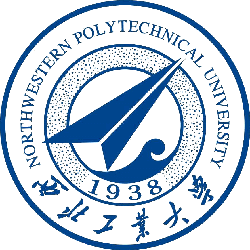
\includegraphics[width=4cm,height=4cm]{NPU-CHINA}
}
\end{center}
\textbf{\\Team Leader}

  张烜槊


\textbf{\\Contact}

  1796164047@qq.com


\textbf{\\A Food & Nutrition Project\\}\begin{spacing}{1.5}

Aflatoxin is a strong carcinogen widely existing in feed crops. Aflatoxin residues in livestock deep-processing products seriously threaten food safety. This project uses \textit{Bacillus subtilis}, which is generally considered safe, as a carrier to assemble aflatoxin degradation proteins, stable-phase promoters and self-cleavage protein. Combined with the selenium-enrichment function of \textit{Bacillus subtilis}, a strain of intelligent \textit{Bacillus subtilis} with self cleavage function, which can simultaneously degrade aflatoxin and enrich selenium, is constructed. Finally, a new, safe and selenium rich high-value feed additive is provided.

黄曲霉素是广泛存在于饲料作物的强致癌物质,牲畜食用后残留于深加工产品的黄曲霉毒素严重威胁食品安全。本项目以普遍认为安全的枯草芽孢杆菌为载体,对黄曲霉毒素降解蛋白、稳定期启动的启动子和自裂解蛋白等元件进行组装。结合枯草芽孢杆菌富硒功能,本项目构建了一株稳定期自裂解的智能黄曲霉毒素降解和富硒枯草芽孢杆菌。最终,提供一种新型、安全、富硒的高值饲料添加剂。\end{spacing}
\\

\url{https://2021.igem.org/Team:NPU-CHINA }\\
\url{https://igem.org/Team.cgi?id=3937 }\\
\url{http://parts.igem.org/wiki/index.php?title=Part:BBa_K3937000 }\\
\url{https://video.igem.org/w/cmwUL7jjCqRsb4gqYh19Bu }\\

\vfill{}









Team of NPU-CHINA will present between      2021/8/28 13:00-14:30   using 腾讯会议 404 469 7665.
\newpage


\subsection{\textcolor{Blu}{ CPU\_CHINA } }
\vspace{5mm}
\begin{center}
\large{
  \textbf{ Construction of MnP-AAO-HFB1 composite system based on CRISPR/dCas9 programmable assembly technology for the oxidation of polyethylene plastic }\\

  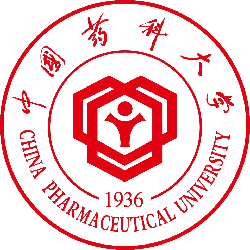
\includegraphics[width=4cm,height=4cm]{CPU_CHINA}
}
\end{center}
\textbf{\\Team Leader}

  郑林雨

  黄子洋


\textbf{\\Contact}

  cpuchina2021@163.com

\textbf{\\An Environment Project\\}\begin{spacing}{1.5}

Examplified by polyethylene, undegradable plastics have a degradation period of hundreds of years under natural conditions, causing severe environmental crisis worldwide. Manganese peroxidase (MnP) uses hydrogen peroxide (H2O2) to produce high-redox-potential Mn3+, possessing a PE-degrading potential. Our project takes MnP as our key PE-degrading enzyme, employs aryl alcohol oxidase (AAO) to provide H2O2 for MnP, and utilizes hydrophobin-1 (HFB1) to increase substrate accessibility, as well as combines SpyCatcher-SpyTag system with CRISPR/dCas9 system to anchor MnP, AAO and HFB1 onto one double-stranded DNA scaffold according to certain spatial order, distance and proportion. The final complex works as a molecular machine that can adhere and degrade PE in a green and swift way.\end{spacing}
\\

\url{https://2021.igem.org/Team:CPU\_CHINA }\\
\url{https://igem.org/Team.cgi?id=3853 }\\
\url{http://parts.igem.org/wiki/index.php?title=Part:BBa_K3853000 }\\
\url{https://video.igem.org/w/sHeaf3vk8E8Rv8bUy5dcb3 }\\

\vfill{}









Team of CPU\_CHINA will present between   2021/8/27 17:00-18:30      using 腾讯会议 404 469 7665.
\newpage


\subsection{\textcolor{Blu}{ XJTLU-CHINA } }
\vspace{5mm}
\begin{center}
\large{
  \textbf{ Dr. Phage }\\

  
\includegraphics[width=4cm,height=4cm]{XJTLU-CHINA}
}
\end{center}
\textbf{\\Team Leader}

  韩欣研


\textbf{\\Contact}

  igem@xjtlu.edu.cn


\textbf{\\A Diagnostics Project\\}\begin{spacing}{1.5}

Our project is to use edited phages containing specific protein-coding genes to infect and lyse bacteria and release the transfected exogenous protein “luxR”, which can then activate downstream cell-free gene circuit and generate visual signal. At that time, the edited phage will not be assembled as the gene of related key protein is cleaved. The downstream circuit outputs binary signals indicating the bacteria concentration meets the national standard or not.\end{spacing}
\\

\url{https://2021.igem.org/Team:XJTLU-CHINA }\\
\url{https://igem.org/Team.cgi?id=4054 }\\
\url{http://parts.igem.org/wiki/index.php?title=Part:BBa_K4054000 }\\
\url{https://video.igem.org/w/9j3Nw6jSXViYmAEkbKJ2D2 }\\

\vfill{}









Team of XJTLU-CHINA will present between        2021/8/28 17:00-18:30 using 腾讯会议 404 469 7665.
\newpage


\subsection{\textcolor{Blu}{ CSU\_CHINA } }
\vspace{5mm}
\begin{center}
\large{
  \textbf{ Sweet Guard }\\

  
\includegraphics[width=4cm,height=4cm]{CSU_CHINA}
}
\end{center}
\textbf{\\Team Leader}

  王泽元

  赵星钧


\textbf{\\Contact}

  308970567@qq.com


\textbf{\\A Therapeutics Project\\}\begin{spacing}{1.5}

Our project aims to find a new method of treating type 1 diabetes with the help of synthetic biology. Our engineered cells will be implanted subcutaneously by mature embedding technology. Blue light activates the automatic insulin production pathway in the cell, meanwhile, its sensation of insulin concentration acts as a detector to cut off the pathway in time to ensure safety.\end{spacing}
\\

\url{https://2021.igem.org/Team:CSU\_CHINA }\\
\url{https://igem.org/Team.cgi?id=3734 }\\
\url{http://parts.igem.org/wiki/index.php?title=Part:BBa_K3734000 }\\
\url{https://video.igem.org/w/ggEtsPspZBPGat7y4GyWbB }\\

\vfill{}









Team of CSU\_CHINA will present between    2021/8/28 8:30-10:00     using 腾讯会议 404 469 7665.
\newpage


\subsection{\textcolor{Blu}{ NJMU-China } }
\vspace{5mm}
\begin{center}
\large{
  \textbf{ Stairway to starlight: Maternal prevention and offspring treatment of autism induced by maternal infection during pregnancy }\\

  
\includegraphics[width=4cm,height=4cm]{NJMU-China}
}
\end{center}
\textbf{\\Team Leader}

  姜璇玮


\textbf{\\Contact}

  wangshuyu2332@163.com


\textbf{\\A Therapeutics Project\\}\begin{spacing}{1.5}

Autism is the fastest-growing developmental disability. According to American CDC, prevalence of autism in the U.S. has increased from 1 in 68 births in 2010 to 1 in 54 births in 2020. Although autism is a biological disorder, it is primarily treated through education and behavioral services, with medication as an important adjunct. However, to date, there is no effective drug to treat ASD. Apart from genetic factors, the protentially dangerous environmental factors to the maternal generation, such as Maternal immune activation(MIA) and Gestational diabetes mellitus (GDM), can also be the cause of ASD. According to the gut-brain axis theory, whether it is maternal immune activation or genetic factors, the etiologies of autism are all related to the gut microbiome. The gut microbiome interacts intimately with the intestins. And CNS deseases such as ASD or stroke can modify the composition of the gut microbiome, leading to a vicious cycle where gut dysbiosis exacerbates the neuroimmune response and aggravates brain pathology and behavior.

Aiming at using synthetic biology to prevent and treat autism through gut-brain axis, our experimental designed involves two parts: prevention in the maternal generation and treatment in the fetal generation. Epidemiological studies suggest that, in humans, fetus' exposure to maternal inflammation increases the likelihood of autism spectrum disorder. When the immune system of a will-be-mother is activated due to infections or autoinflammatory syndromes, the Th17 and Treg cells in her bowel will lose their balance and inflammatory factors, such as IL-17, can then be transferred across the placental barrier to harm the nervous system of the fetus. In this case, her child will have an increased risk of neurodevelopmental disorders. So we decided to develop a probiotic strain of \textit{E. coli} as a novel, self-tuning “drug” for pregnant women to reudce the risk of autism in the offspring. As for treatment in the fetal generation, we attempted to code secretable oxytocin, which can be transported to the central nervous system through the gut-brain axis.

Children with ASDs are also what we call ‘Children From the Star’. They are stars twinkling in the distant sky, all waiting for their time to drop on the earth but happening to be trapped in a bottle. And when the trapped one falls into a human's bosom, the lady becomes his or her dear mother. When they grow up, they find it hard to make friends with other ‘normal’ kids. So the little one stays in his or her own planet, with nobody having ever landed on their planets and certain about what their planets are like. Our project aims at building up a stairway to the starlight, using engineering probiotics to prevent autism caused by maternal infection during pregnancy and treat children, thus structuring a way to health for the ‘Children From the Star’.\end{spacing}
\\

\url{https://2021.igem.org/Team:NJMU-China }\\
\url{https://igem.org/Team.cgi?id=3873 }\\
\url{http://parts.igem.org/wiki/index.php?title=Part:BBa_K3873000 }\\
\url{https://video.igem.org/w/wHC2UUhKevLbbU7zfEz4SC }\\

\vfill{}









Team of NJMU-China will present between    2021/8/28 8:30-10:00     using 腾讯会议 404 469 7665.
\newpage


\subsection{\textcolor{Blu}{ NWU-CHINA-B } }
\vspace{5mm}
\begin{center}
\large{
  \textbf{ The transformation journey of ginsenosides }\\

  
\includegraphics[width=4cm,height=4cm]{NWU-CHINA-B}
}
\end{center}
\textbf{\\Team Leader}

  李佳程


\textbf{\\Contact}

  1419576562@qq.com


\textbf{\\A Manufacturing Project\\}\begin{spacing}{1.5}

Ginsenosides, as active components of ginseng, have many pharmacological activities. Among them, ginsenoside CK has been widely studied for its excellent biological activities such as treating diabetes, anti-tumor, anti-inflammatory and anti-aging. However, CK almost does not exist in natural ginseng and can be produced by ginsenoside Rb1 through enzymatic conversion. In order to improve CK production, this project expressed β -glucoside enzyme derived from sulphurite leaf vulcanization bacteria in Pichia pastoris GS115 and applied it to deglycosylation of Rb1 and production of CK.

In this project, the SS-bgly gene derived from Sulfolobus solfataricus will be highly expressed in pichia coli system after codon optimization, and the enzymatic reaction conditions for the transformation of ginsenoside substrate Rb1 to CK from SS-bgly will be explored. Under the optimized enzymatic reaction conditions, the recombinant SS-bgly can transform ginsenoside Rb1 with higher substrate concentration into CK, which is conducive to the large-scale production of CK.\end{spacing}
\\

\url{https://2021.igem.org/Team:NWU-CHINA-B }\\
\url{https://igem.org/Team.cgi?id=3779 }\\
\url{http://parts.igem.org/wiki/index.php?title=Part:BBa_K3779000 }\\
\url{https://video.igem.org/w/xvh9pD5AF4uPJ9JthZovEX }\\

\vfill{}









Team of NWU-CHINA-B will present between  2021/8/27 15:00-16:30       using 腾讯会议 404 469 7665.
\newpage


\subsection{\textcolor{Blu}{ USTC } }
\vspace{5mm}
\begin{center}
\large{
  \textbf{ AD early diagnosis }\\

  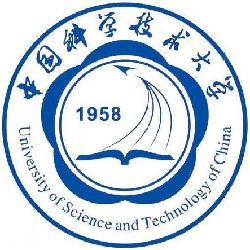
\includegraphics[width=4cm,height=4cm]{USTC}
}
\end{center}
\textbf{\\Team Leader}

  曹耀中

  张广为

  薛睿豪


\textbf{\\Contact}

  ch0703@mail.ustc.edu.cn


\textbf{\\A Diagnostics Project\\}\begin{spacing}{1.5}

It's reported that Tau protein level in serum may indicate AD progress. Thus, we devised a new-concept \textit{in vitro} Tau detection method for early AD diagnosis, depending on the specific binding between aptamers and Tau proteins. First, a molecular switch transfers the aptamer-protein binding signal to a downstream signal pathway. Second, the downstream signal pathway amplifies the signal exponentially to a detectable level. Our method has more convenience, lower cost and higher specificity and sensitivity.\end{spacing}
\\

\url{https://2021.igem.org/Team:USTC }\\
\url{https://igem.org/Team.cgi?id=3912 }\\
\url{http://parts.igem.org/wiki/index.php?title=Part:BBa_K3912000 }\\
\url{https://video.igem.org/w/9KNJ1sXNyDKTH3S8sBY6vE }\\

\vfill{}









Team of USTC will present between        2021/8/28 17:00-18:30 using 腾讯会议 404 469 7665.
\newpage


\subsection{\textcolor{Blu}{ SJTU-Software } }
\vspace{5mm}
\begin{center}
\large{
  \textbf{ An intelligent platform for DNA nano machine contriving }\\

  
\includegraphics[width=4cm,height=4cm]{SJTU-Software}
}
\end{center}
\textbf{\\Team Leader}

  胡远洁


\textbf{\\Contact}

  rosesilver@sjtu.edu.cn


\textbf{\\A Software Project\\}\begin{spacing}{1.5}

The current DNA computation and its application are still in the laboratory stage,which is difficult to apply DNA computation for researchers without rich professional knowledge. This project aims to build a comprehensive dynamic DNA computing work platform to assist scientific researchers in accelerating the progress of research. This platform integrates bioinformatics analysis, machine learning models and molecular dynamics simulation to achieve design guidance and predictive simulation of dynamic DNA computation sequences. It can be applied to low-cost, non-invasive, and conventional early cancer screening.\end{spacing}
\\

\url{https://2021.igem.org/Team:SJTU-Software }\\
\url{https://igem.org/Team.cgi?id=3741 }\\
\url{http://parts.igem.org/wiki/index.php?title=Part:BBa_K3741000 }\\


\vfill{}









Team of SJTU-Software will present between 2021/8/27 13:00-14:30        using 腾讯会议 404 469 7665.
\newpage


\subsection{\textcolor{Blu}{ Tongji\_Software } }
\vspace{5mm}
\begin{center}
\large{
  \textbf{ Phage\_MAP }\\

  
\includegraphics[width=4cm,height=4cm]{Tongji_Software}
}
\end{center}
\textbf{\\Team Leader}

  卓正一

  汪明杰

  赵艳萍


\textbf{\\Contact}

  zhaoyanping@tongji.edu.cn


\textbf{\\A Software Project\\}\begin{spacing}{1.5}

Based on the interactions of phage and bacteria according to consistent sequences, we try to establish an interactive map called Phage-MAP, which demonstrates the potentially corresponding relationship between phage and bacteria. It is pretty conducive to select specific phage or phage combinations to achieve precise treatment to a certain bacterium.\end{spacing}
\\

\url{https://2021.igem.org/Team:Tongji\_Software }\\
\url{https://igem.org/Team.cgi?id=3847 }\\
\url{http://parts.igem.org/wiki/index.php?title=Part:BBa_K3847000 }\\
\url{https://video.igem.org/w/hCHD2AAitBnumnyUab5LDZ }\\

\vfill{}









Team of Tongji\_Software will present between 2021/8/27 13:00-14:30        using 腾讯会议 404 469 7665.
\newpage


\subsection{\textcolor{Blu}{ Fudan } }
\vspace{5mm}
\begin{center}
\large{
  \textbf{ Candicamera }\\

  
\includegraphics[width=4cm,height=4cm]{Fudan}
}
\end{center}
\textbf{\\Team Leader}

  兰心


\textbf{\\Contact}

  igem@fudan.edu.cn


\textbf{\\A Diagnostics Project\\}\begin{spacing}{1.5}

The yeast \textit{Candida albicans} causes diseases as vaginal infections, affecting up to 75\% of women. By applying synthetic biology gene circuits entailing the T7 RNA polymerase inhibitor, team Fudan lowers the cost of detection of \textit{Candida albicans} and develop a new product —— Candicamera. Candicamera allows rapid and efficient diagnosis of \textit{Candida albicans} in resource-limited settings and for point-of-care analysis.\end{spacing}
\\

\url{https://2021.igem.org/Team:Fudan }\\
\url{https://igem.org/Team.cgi?id=3790 }\\
\url{http://parts.igem.org/wiki/index.php?title=Part:BBa_K3790000 }\\
\url{https://video.igem.org/w/7nsVni1Fc2HXbewZ6U3quV }\\

\vfill{}









Team of Fudan will present between        2021/8/28 17:00-18:30 using 腾讯会议 404 469 7665.
\newpage


\subsection{\textcolor{Blu}{ ZJU-China } }
\vspace{5mm}
\begin{center}
\large{
  \textbf{ 肝卫士: 基于增强型溶瘤腺病毒的特异性肝癌靶向治疗\\ Liver Guard: Precise therapy of hepatocellular carcinoma based on engineered oncolytic adenovirus }\\

  
\includegraphics[width=4cm,height=4cm]{ZJU-China}
}
\end{center}
\textbf{\\Team Leader}

  吴浩然


\textbf{\\Contact}

  haoranwu@zju.edu.cn


\textbf{\\A Therapeutics Project\\}\begin{spacing}{1.5}

Oncolytic virus (OV) is a promising method to treat hepatocellular carcinoma, yet it has not been widely used clinically due to low infection efficiency, insufficient specificity, compromised intertumoral transmission and etc. Our project designed a genetically modified adenovirus using synthetic biology approach to overcome current problems with oncolytic virus. We also enables engineered adenovirus to escape from immunity trap with immunocamouflage, which increases the titre of viral infection. It is highly hoped that our project can give a new insight into precise oncolytic treatment of HCC.

溶瘤病毒疗法是目前治疗癌症的新途径,但由于感染效率低、特异性不足、瘤内传播障碍等问题而未在临床上得到广泛应用。本项目通过对腺病毒进行合成生物学改造,增强病毒对肝癌细胞的特异性侵染、复制及瘤内传播,并加入免疫伪装机制,减少由于机体免疫造成的溶瘤病毒清除,实现原发性肝癌高效靶向治疗,为癌症的精准治疗提供科学依据。\end{spacing}
\\

\url{https://2021.igem.org/Team:ZJU-China }\\
\url{https://igem.org/Team.cgi?id=3730 }\\
\url{http://parts.igem.org/wiki/index.php?title=Part:BBa_K3730000 }\\


\vfill{}









Team of ZJU-China will present between    2021/8/28 8:30-10:00     using 腾讯会议 404 469 7665.
\newpage


\subsection{\textcolor{Blu}{ NWU-CHINA-A } }
\vspace{5mm}
\begin{center}
\large{
  \textbf{ Construction of the \textit{Escherichia coli} two-cell system for monarch violet dye production }\\

  
\includegraphics[width=4cm,height=4cm]{NWU-CHINA-A}
}
\end{center}
\textbf{\\Team Leader}

  高琪

  王若舟


\textbf{\\Contact}

  2991088806@qq.com


\textbf{\\A New Application Project\\}\begin{spacing}{1.5}

Tyrian purple, also known as, 6,6-dibromoindigo, is a kind of natural pigment with a long history of production and application, which was always been preferred by the royal. In addition to its value in history and culture, as a kind of novel biocompatible semiconductor it also receive much attention. However, due to natural yield little, difficulty in chemosynthesis and the potential pollution, its high yield production hasn't been realized. Therefore, we plan to implement a two-cell reaction by spatiotemporally separating the two consecutive procedures of the production, so that the enzyme in tyrian purple metabolic pathway could achieve its highest efficiency. Moreover, we can choose some gene expression regulatory parts to improve the high-yield and high-purity dual cell system.

帝王紫,即6,6-二溴靛蓝,是拥有悠久生产与应用历史的天然染料,历史上一直为统治阶级所钟爱,除其承载的历史文化价值外,帝王紫作为新型生物相容性导体,在半导体材料中也倍受瞩目。但由于其天然产量少,化学合成困难且存在环境污染,迄今未能实现高产。本项目拟采用双细胞系统,进行生产时空分离,以达到帝王紫代谢通路中相关酶的最高利用效率,并严格筛选基因表达调控原件,构建帝王紫高纯度、高产量双细胞体系。\end{spacing}
\\

\url{https://2021.igem.org/Team:NWU-CHINA-A }\\
\url{https://igem.org/Team.cgi?id=3722 }\\
\url{http://parts.igem.org/wiki/index.php?title=Part:BBa_K3722000 }\\
\url{https://video.igem.org/w/kE9VkEAnLpHz1s3nnFtXhy }\\

\vfill{}









Team of NWU-CHINA-A will present between      2021/8/28 13:00-14:30   using 腾讯会议 404 469 7665.
\newpage


\subsection{\textcolor{Blu}{ SZU-China } }
\vspace{5mm}
\begin{center}
\large{
  \textbf{ 针对炎症性肠病的个性化定制辅剂生产工厂 }\\

  
\includegraphics[width=4cm,height=4cm]{SZU-China}
}
\end{center}
\textbf{\\Team Leader}

  陈睿越

  孙一帆

  余思洋


\textbf{\\Contact}

  913385760@qq.com


\textbf{\\A Manufacturing Project\\}\begin{spacing}{1.5}

炎症性肠病(IBD)存在发病周期长,难彻底根治,具有较高的潜在癌变风险等问题,一经患病会对患者的生活质量造成极大影响,持续性的临床治疗和全方位的健康干预是抑制和减轻病症的最佳手段。目前,全球有超过 1000 万人患有 IBD 及相关疾病,预计到2025年,我国炎症性肠病患者也将达到150万人。2021年SZU-China团队与行业领先的肠道微生物AI制药公司合作,希望利用基因改造的工程菌对已被证实的四个潜在致病靶点进行“鸡尾酒式”辅剂治疗,以冻干肠溶制剂作为最终产品形式,探索从患者粪便采样分析、靶点筛选、设计制药方案、配比菌种、以及饮食和心理健康关怀等六大环节,以全产业链的视角切入,进行资源整合,尝试构筑个性化治疗生态体系样本。在公众认知层面,我们也将通过多种渠道进行宣传,向公众普及 IBD 疾病知识,补齐公众认知缺失,助力实现“健康中国2030”远景目标及联合国可持续发展目标。\end{spacing}
\\

\url{https://2021.igem.org/Team:SZU-China }\\
\url{https://igem.org/Team.cgi?id=3838 }\\
\url{http://parts.igem.org/wiki/index.php?title=Part:BBa_K3838777 }\\
\url{https://video.igem.org/w/a5tYeSh3GczSACFNgtVFYT }\\

\vfill{}









Team of SZU-China will present between 2021/8/27 13:00-14:30        using 腾讯会议 404 469 7665.
\newpage


\subsection{\textcolor{Blu}{ NJTech\_China } }
\vspace{5mm}
\begin{center}
\large{
  \textbf{ Saving Rose Plan : Design and Construction of Synthetic Microalgae-Yeast Consortia for Biosynthesis of Phenylethanol }\\

  
\includegraphics[width=4cm,height=4cm]{NJTech_China}
}
\end{center}
\textbf{\\Team Leader}

  王宇娇

  章益蜻


\textbf{\\Contact}

  1005172875@qq.com


\textbf{\\A Manufacturing Project\\}\begin{spacing}{1.5}

Phenylethanol has been widely used in cosmetics and other fields owing to its rose aroma. This project chooses \textit{Saccharomyces cerevisiae} as the chassis microorganism, optimizes the phenethylamine pathway of different sources and different expression modes, strengthens the activity of endogenous alcohol dehydrogenase, establishes a yeast-microalgae microbial consortia system based on nutritional complementation and metabolites exchange. The combination with 3D printing microcapsule embedding technology will eventually guide to establish a robust, stable, and controllable artificial microbial consortia system for the green and efficiency phenylethanol biosynthetic.

苯乙醇因具有玫瑰香气而广泛用于化妆品等领域。本项目以酿酒酵母为底盘细胞,通过优化不同来源、不同表达方式的苯乙胺途径;强化内源醇脱氢酶活性;建立基于营养互补、代谢物交换的酵母-微藻双菌体系;结合3D打印微胶囊包埋技术,最终建立系统鲁棒、稳定、可控的苯乙醇绿色高效生物合成的人工双菌体系。\end{spacing}
\\

\url{https://2021.igem.org/Team:NJTech\_China }\\
\url{https://igem.org/Team.cgi?id=3753 }\\
\url{http://parts.igem.org/wiki/index.php?title=Part:BBa_K3753000 }\\
\url{https://video.igem.org/w/hMu8pFLufMJa8c43KBPaqZ }\\

\vfill{}









Team of NJTech\_China will present between 2021/8/27 13:00-14:30        using 腾讯会议 404 469 7665.
\newpage


\subsection{\textcolor{Blu}{ SYSU-CHINA } }
\vspace{5mm}
\begin{center}
\large{
  \textbf{ CircRNA Assembly FacTory }\\

  
\includegraphics[width=4cm,height=4cm]{SYSU-CHINA}
}
\end{center}
\textbf{\\Team Leader}

  李思珺*

  余雅婷

  赵炳喃

  董情


\textbf{\\Contact}

  2395479525@qq.com


\textbf{\\A Foundational Advance Project\\}\begin{spacing}{1.5}

Team SYSU-CHINA this year plans to use Rational-designed circRNA scaffold to handle some practical problems, such as improving the production of biofuel. We choose different RNA binding proteins fused with different proteins of interest by different kinds of linkers, which can bind to specific sites on the circRNA constructed \textit{in vitro}. After debugging, we hope to colocalize a series of related enzymes and accelerate the biochemistry reaction.\end{spacing}
\\

\url{https://2021.igem.org/Team:SYSU-CHINA }\\
\url{https://igem.org/Team.cgi?id=3960 }\\
\url{http://parts.igem.org/wiki/index.php?title=Part:BBa_K3960000 }\\
\url{https://video.igem.org/w/qRfZFj3VJ78Whfhe22CRXc }\\

\vfill{}









Team of SYSU-CHINA will present between     2021/8/28 10:30-12:00    using 腾讯会议 404 469 7665.
\newpage


\subsection{\textcolor{Blu}{ NJU-China } }
\vspace{5mm}
\begin{center}
\large{
  \textbf{ Targeted therapy of asthma by self-assembled small interfering RNA \textit{in vivo} }\\

  
\includegraphics[width=4cm,height=4cm]{NJU-China}
}
\end{center}
\textbf{\\Team Leader}

  陶辰宇


\textbf{\\Contact}

  1171716152@qq.com


\textbf{\\A New Application Project\\}\begin{spacing}{1.5}

Asthma is a chronic respiratory disease estimated to affect more than 339 million people worldwide. People suffering from asthma can only use different levels of ICS or ICS-LABA to prevent exacerbations and control symptoms. We focus on type 2 inflammation in bronchus, which is common but a key contributor to asthma. Our scheme is to take advantage of RNAi therapy to target TSLP and GATA3 to degrade their expression of mRNA and consequently improve asthma situations. During this process, we use a self-assembled siRNA delivery system where we enclose the siRNAs with exosomes to inhibit the above genes' translation and to subsequently prevent downstream toxicity and immunogenicity, which is superior to the otherwise exogenously pre-assembled systems. Meanwhile, we connected with our community through human practices to raise awareness of asthma. To ensure our sustainable impact, we held a regional meetup and founded an organization called the Nanjing iGEM Association (NIA).\end{spacing}
\\

\url{https://2021.igem.org/Team:NJU-China }\\
\url{https://igem.org/Team.cgi?id=3756 }\\
\url{http://parts.igem.org/wiki/index.php?title=Part:BBa_K3756000 }\\
\url{https://video.igem.org/w/sSH24uc7dcnchgMLWEaSdy }\\

\vfill{}









Team of NJU-China will present between       2021/8/28 15:00-16:30  using 腾讯会议 404 469 7665.
\newpage


\subsection{\textcolor{Blu}{ CSU\_CHINA(iDEC) } }
\vspace{5mm}
\begin{center}
\large{
  \textbf{ Peplib generator is all you need }\\

  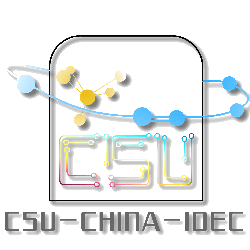
\includegraphics[width=4cm,height=4cm]{CSU_CHINA(iDEC)}
}
\end{center}
\textbf{\\Team Leader}

  张彦哲


\textbf{\\Contact}

  seanpeldomzhang@qq.com


An Information Processing Project\\}\begin{spacing}{1.5}

Long and costly process lies between target discovery and drug approval. So, in recent decade, pharmaceutical corporations have been using distributed AI models to assist in accelerating the R & D cycle and reducing costs in multiple stages, yet the average cost is still increasing. For peptide drugs, that multiple stages come as follows: data collection, feature representation, AI model construction, rational design, peptide library construction, affinity prediction, animal model experimental test, clinical test and the last approval. By developing a general and integrated AI model of peptide directed evolution, we can generate an optimized peptide virtual library from the target protein in one step instead, only to be waited for the next animal model experiment. Based on the idea of generation antagonism networks (GAN) , we developed and combined multi-dimensional discriminant networks and a sequence generation network to compete with each other, quickly and finely generate multiple optimal solutions in the protein sequence space under the constraints of given targets and expected multi properties, as new potential peptide drugs, to achieve the goal of one-step generation of the most promising sequence library.\end{spacing}
\\

\vfill{}









Team of CSU\_CHINA(iDEC) will present between 2021/8/27 13:00-14:30        using 腾讯会议 404 469 7665.
\newpage


\subsection{\textcolor{Blu}{ SCUT-China } }
\vspace{5mm}
\begin{center}
\large{
  \textbf{ Screening and Engineering of Promoters to Improve the Production of Nootkatone in \textit{Saccharomyces cerevisiae} }\\

  
\includegraphics[width=4cm,height=4cm]{SCUT-China}
}
\end{center}
\textbf{\\Team Leader}

  曾徽


\textbf{\\Contact}

  814856333@qq.com


\textbf{\\A Manufacturing Project\\}\begin{spacing}{1.5}

Located in the humid and rainy south, the problem of mosquito repellent has been the concern of Guangzhou people. Mosquitoes are not only annoying, but what's more, they can also spread various diseases, such as dengue fever, which is a great threat to human health. So, in tropical and subtropical areas, mosquito repellant products are in great demand. Nootkatone is a new mosquito repellent ingredient reported by EPA, which offers increased safety and stability, but high cost has caused production limitations. We plan to achieve high yield of nootkatone precursor (valencene) through promoter engineering. Firstly, we establish a promoter pool of \textit{Saccharomyces cerevisiae}. Then, we obtain stronger promoters that support high expression to synthesize valencene for most fermentation phases via alternation and recombination of upstream activated sequence (UAS). We establishe nucleosome affinity model to optimize the UAS of the hybrid promoter, so as to maximize the efficiency of the transcription and reduce production costs , which ultimately help achieve higher market shares of nootkatone and let more people benefit from it.

地处潮湿多雨的南方,驱蚊问题一直备受广州人民的关注。蚊子不仅让人心烦意乱,更可怕的是,蚊子还会传播各种疾病,如对人类的健康造成极大威胁的登革热等。因此在热带和亚热带地区,驱蚊产品有着很大的市场需求。圆柚酮是 EPA报道的新型驱蚊成分,具有更高的安全性和稳定性,但高昂的成本造成了生产限制。我们通过酿酒酵母的启动子工程实现圆柚酮前体(瓦伦烯)的高产量。我们首先建立酿酒酵母启动子库,并通过不同启动子的上游激活序列(UAS)的组合,获得了发酵早期和晚期均支持高表达的杂合启动子。接着我们建立核小体亲和力模型,对启动子进行优化,使转录效率最大化,从而提高诺卡酮前体(瓦伦烯)的生产量,降低生产成本,最终使圆柚酮获得更高的市场份额,让更多人受益。\end{spacing}
\\

\url{https://2021.igem.org/Team:SCUT-China }\\
\url{https://igem.org/Team.cgi?id=3772 }\\
\url{http://parts.igem.org/wiki/index.php?title=Part:BBa_K3772000 }\\
\url{https://video.igem.org/w/pPc11iq9W2s51axSG2J2bD }\\

\vfill{}









Team of SCUT-China will present between 2021/8/27 13:00-14:30        using 腾讯会议 404 469 7665.
\newpage


\subsection{\textcolor{Blu}{ Tongji\_China } }
\vspace{5mm}
\begin{center}
\large{
  \textbf{ LOOK! }\\

  
\includegraphics[width=4cm,height=4cm]{Tongji_China}
}
\end{center}
\textbf{\\Team Leader}

  张艺瀛

  胡红娟


\textbf{\\Contact}

  1950187@tongji.edu.cn


\textbf{\\An Environment Project\\}\begin{spacing}{1.5}

Since the implementation of household garbage sorting regulations in Shanghai, the amount of food waste has reached a peak. However, the health problems and unpleasant smell caused by odor generated from food waste have aroused attention not only in Shanghai but also in other areas. This year, Tongji China launches the “LOOK!” project to solve the odor of food waste. We construct two kinds of bioengineered \textit{E. coli} to absorb hydrogen sulfide and ammonia, which are the two main ingredients in the odor. One uses enzymes related to sulfide oxidazation(Sqr, Sdo, AprBA and Sat), converting hydrogen sulfide to sulfate, while the other uses enzymes related to ammonia oxidazation (AMO, HAO and NOD), converting ammonia to nitrate. Besides, a three-gear adjustable kill switch based on the concentration of H2S and NH3 will be added to ensure biosafety. Also, we'll optimize our pathway by high throughput screening and machine learning. We've conducted several rounds of Human Practices to gather suggestions from various aspects to improve our project. With such efforts, we hope that the problems the odor has brought to residents as well as waste disposal industries and their downstream industries can be solved in the future.\end{spacing}
\\

\url{https://2021.igem.org/Team:Tongji\_China }\\
\url{https://igem.org/Team.cgi?id=3823 }\\
\url{http://parts.igem.org/wiki/index.php?title=Part:BBa_K3823000 }\\
\url{https://video.igem.org/w/1wRujvsqeZpjSg33fu1fQd }\\

\vfill{}









Team of Tongji\_China will present between   2021/8/27 17:00-18:30      using 腾讯会议 404 469 7665.
\newpage


\subsection{\textcolor{Blu}{ XJTU-China } }
\vspace{5mm}
\begin{center}
\large{
  \textbf{ Tryptophan iDream }\\

  
\includegraphics[width=4cm,height=4cm]{XJTU-China}
}
\end{center}
\textbf{\\Team Leader}

  陈泓宇

  姚海龙


\textbf{\\Contact}

  2696331468@qq.com


\textbf{\\A Food & Nutrition Project\\}\begin{spacing}{1.5}

Tryptophan, an essential amino acid, can be used as a food addictive to treat certain mental problems like insomnia and depression that greatly affect the life quality of the patients especially in modern society. Although the tryptophan supplied to the market is not shortage due to the mass production via chemical synthesis, patients of insomnia or depression still eager to get access to such chemicals or health products more conveniently. In other words, a tryptophan-producing, domestic and portable device is a latent and potential trend for the patients to get rid of redundant steps in purchasing tryptophan and certainly, to treat insomnia and depression.

In our project, \textit{E. coli} is adapted to construct a brand new strain whose regular proliferation and tryptophan biosynthesis are separated and controlled through a bistable control system, i.e. toggle switch, without affecting the viability of the cells. If possible, we hope to build the device to produce and purify the tryptophan based on our edited strain.

In our toggle switch, faster cell proliferation is expected to be witnessed under the induction of IPTG, while paused proliferation and elevated tryptophan yield would be observed after a growing temperature shift to over 42 degree. As for the circuit, critical genes for either \textit{E. coli} proliferation or tryptophan synthesis are retrieved and picked on the basis of previously published research. Ultimately, pykA (for proliferation) and aroG&trpAB (for trp synthesis) were chosen to composite the toggle switch together with other necessary cis-acting elements. pykA encodes pyruvate kinase A in \textit{E. coli}, which catalyzes the formation of pyruvate in the last step of glycolysis. Thus, the overexpression of pykA via exogenous plasmids is expected to result in an increase of pyruvate utilized by TCA cycle to produce additional NADH and ATP to support cell growth and division. However, glycolysis branches off at phosphoenolpyruvate (PEP) because AroG catalyzes the formation of DAHP from PEP, and eventually tryptophan is synthesized due to a set of successive enzymes including trpAB. Hence, overexpression of aroG and trpAB elevates the tryptophan yield level but on the other hand affects the cell proliferation.\end{spacing}
\\

\url{https://2021.igem.org/Team:XJTU-China }\\
\url{https://igem.org/Team.cgi?id=3832 }\\
\url{http://parts.igem.org/wiki/index.php?title=Part:BBa_K3832000 }\\
\url{https://video.igem.org/w/j5E8xUwTq41LHSE7ivATE8 }\\

\vfill{}









Team of XJTU-China will present between      2021/8/28 13:00-14:30   using 腾讯会议 404 469 7665.
\newpage


\subsection{\textcolor{Blu}{ CAU\_China } }
\vspace{5mm}
\begin{center}
\large{
  \textbf{ SSR: Saline-alkaline Soil Restorer }\\

  
\includegraphics[width=4cm,height=4cm]{CAU_China}
}
\end{center}
\textbf{\\Team Leader}

  李明阳

  杨飞月


\textbf{\\Contact}

  393811901@qq.com


\textbf{\\An Environment Project\\}\begin{spacing}{1.5}

Saline-alkali soil is unfavorable to crop growth. γ-polyglutamic acid, aka γ-PGA, is formed by glutamic acid. CAU\_China hopes to treat the saline-alkali land through γ-PGA by soil bacteria Corynebacterium glutamicum using synthetic biology. We transfer the related genes from Bucillus subtilis into C.glutamicum to make it use glutamate to produce γ-PGA. We apply a composite kill-switch to kill our bacteria when both the ionic strength and pH of the soil decrease to an expected level.\end{spacing}
\\

\url{https://2021.igem.org/Team:CAU\_China }\\
\url{https://igem.org/Team.cgi?id=3796 }\\
\url{http://parts.igem.org/wiki/index.php?title=Part:BBa_K3796000 }\\
\url{https://video.igem.org/w/mpDErSEW314zVRoSwMWm1j }\\

\vfill{}









Team of CAU\_China will present between   2021/8/27 17:00-18:30      using 腾讯会议 404 469 7665.
\newpage


\subsection{\textcolor{Blu}{ Jilin\_China } }
\vspace{5mm}
\begin{center}
\large{
  \textbf{ Mosquiet }\\

  
\includegraphics[width=4cm,height=4cm]{Jilin_China}
}
\end{center}
\textbf{\\Team Leader}

  马健哲

  曹天欣


\textbf{\\Contact}

  1759755543@qq.com


\textbf{\\A New Application Project\\}\begin{spacing}{1.5}

Our project aims to design a new, harmless mosquito-killing device. The device produces l-lactic acid, acetic acid, ammonia to attract mosquitoes, and combines with high voltage electric net to achieve the purpose of trapping and killing mosquitoes. We also perform quorum sensing and acid response dynamic regulation to control key genes and use a suicide switch to prevent the leakage of bacteria.\end{spacing}
\\

\url{https://2021.igem.org/Team:Jilin\_China }\\
\url{https://igem.org/Team.cgi?id=3883 }\\
\url{http://parts.igem.org/wiki/index.php?title=Part:BBa_K3883000 }\\
\url{https://video.igem.org/w/4uBBBiJEE5rtrG2H5s8rrh }\\

\vfill{}









Team of Jilin\_China will present between       2021/8/28 15:00-16:30  using 腾讯会议 404 469 7665.
\newpage


\subsection{\textcolor{Blu}{ Nanjing\_NFLS } }
\vspace{5mm}
\begin{center}
\large{
  \textbf{ Antibiotic Killer }\\

  
\includegraphics[width=4cm,height=4cm]{Nanjing_NFLS}
}
\end{center}
\textbf{\\Team Leader}

  陆佳睿


\textbf{\\Contact}

  2025293160@qq.com


\textbf{\\A High-School Energy Project\\}\begin{spacing}{1.5}

四环素污染是目前抗生素污染中的重大问题。电芬顿法降解抗生素有高效和便捷的优点。今年,我们队伍想通过微生物燃料电池降解四环素中的金霉素。通过过表达rhlI和rhlR基因,我们能够增强阳极微生物间的群体感应,从而加快生物膜成膜速度,提高微生物燃料电池的效率。同时,在阴极室,我们通过铁基修饰,使阴极发生电芬顿反应,降解金霉素。由于微生物燃料电池效率的提高,降解效率也显著增加。\end{spacing}
\\

\url{https://2021.igem.org/Team:Nanjing\_NFLS }\\
\url{https://igem.org/Team.cgi?id=3964 }\\
\url{http://parts.igem.org/wiki/index.php?title=Part:BBa_K3964000 }\\


\vfill{}









Team of Nanjing\_NFLS will present between  2021/8/27 15:00-16:30       using 腾讯会议 404 469 7665.
\newpage


\subsection{\textcolor{Blu}{ UESTC-China } }
\vspace{5mm}
\begin{center}
\large{
  \textbf{ Deink the dark }\\

  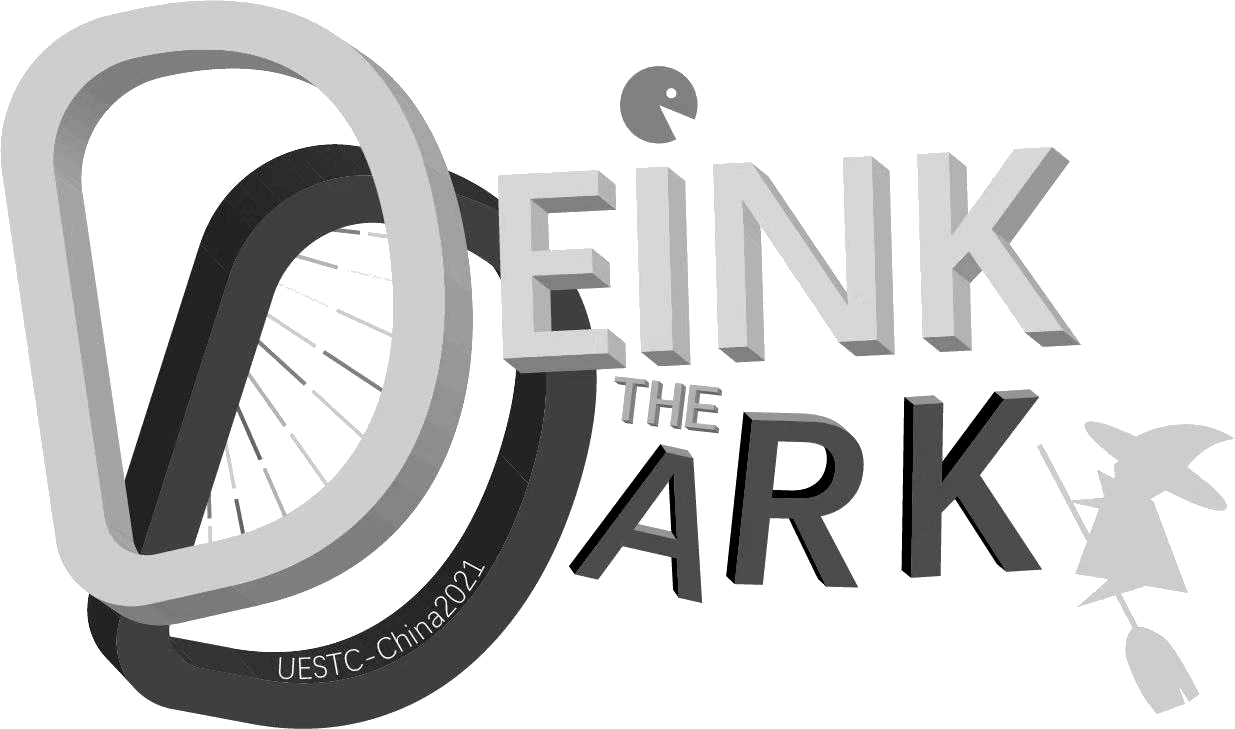
\includegraphics[width=4cm,height=4cm]{UESTC-China}
}
\end{center}
\textbf{\\Team Leader}

  周颖

  胡雨薇


\textbf{\\Contact}

  249468856@qq.com


\textbf{\\A New Application Project\\}\begin{spacing}{1.5}

CEPI (Confederation of European Paper Industries) has reported that the recycling rate of office waste paper (OWP) is dramatically low (12.9\%) in Europe though this kind of paper has a high value to regenerate. In addition, our market research has produced similar results. We find that cellulase, xylanase, lipase, and laccase will allow biodeinking to occur, by helping the ink detach from the waste paper and decomposing hazardous substances. In our project, we designed a new surface assembly of a functional cellulosome by using a synthetic yeast consortium, Pichia pastoris. The basic design of the consortiums consisted of five different engineered yeast strains are capable of displaying a trifunctional scaffolding carrying two divergent cohesion domains from Clostridium thermocellum and Clostridium cellulolyticum in proportion 2:1, secreting the two corresponding dockerin-tagged cellulase and xylanase and the other two enzymes named lipase and laccase. The secreted cellulase and xylanase are docked onto the displayed Scaffolding in a highly organized manner based on the specific interaction of the two cohesin-dockerin pairs, resulting in the assembly of a functional cellulosome on the yeast surface. To bring our idea to the real world, we design a paper recycle machine (Deinker), mainly including the transmission part, the enzyme liquid smearing part, the deinking part, and the paper drying part. When using, the paper only needs to be fixed on the cardboard, and the deinking can be started with one button on the touch screen. Finally, you can get a piece of white paper that can be used again. Through this device, the office waste paper will be reborn. In addition, mathematical models are built for improving experiments, hardware, and implementation: A model for specific protein structure prediction and molecular docking; a model for predicting the optimum ratio and reaction conditions of various enzymes; a model for ink recognition on the paper surface; a model for improving the drying efficiency of paper by increasing the performance of the machine; a decision-making model of optimal placement of deinker in different application scenarios. Prospectively, our research project can not only recycle office paper but also reduce the cost of printing errors and prevent the leakage of information. Deink the dark make the world better with less tree cut.\end{spacing}
\\

\url{https://2021.igem.org/Team:UESTC-China }\\
\url{https://igem.org/Team.cgi?id=3819 }\\
\url{http://parts.igem.org/wiki/index.php?title=Part:BBa_K3819000 }\\
\url{https://video.igem.org/w/rWSvb9mKgsA5v4XSAjizQT }\\

\vfill{}









Team of UESTC-China will present between       2021/8/28 15:00-16:30  using 腾讯会议 404 469 7665.
\newpage


\subsection{\textcolor{Blu}{ BNU-China } }
\vspace{5mm}
\begin{center}
\large{
  \textbf{ A Cheater-proof System }\\

  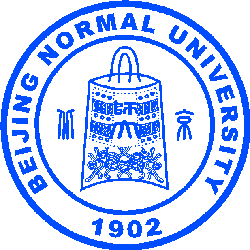
\includegraphics[width=4cm,height=4cm]{BNU-China}
}
\end{center}
\textbf{\\Team Leader}

  唐悦

  陈乐然

  李雨默


\textbf{\\Contact}

  1604942361@qq.com


\textbf{\\A Manufacturing Project\\}\begin{spacing}{1.5}

In some natural colonies, microorganisms cooperate with each other by sharing essential substances. However, some “cheaters” who use public resources without synthesis emerge in the process of evolution. When cheaters appear in the industrial production, it may cause a loss in both quality and quantity of the products. To solve this problem, BNU-China develops a “cheater-proof” platform for industrial production by introducing automatically switchable “guards” into the system.\end{spacing}
\\

\url{https://2021.igem.org/Team:BNU-China }\\
\url{https://igem.org/Team.cgi?id=3805 }\\
\url{http://parts.igem.org/wiki/index.php?title=Part:BBa_K3805000 }\\
\url{https://video.igem.org/w/u5dDYRwud2bYMRoED2kfNa }\\

\vfill{}









Team of BNU-China will present between  2021/8/27 15:00-16:30       using 腾讯会议 404 469 7665.
\newpage


\subsection{\textcolor{Blu}{ BIT-China } }
\vspace{5mm}
\begin{center}
\large{
  \textbf{ Creative Tasting Officer -- Smart yeast knows your taste: Customized plant-derived food seasonings }\\

  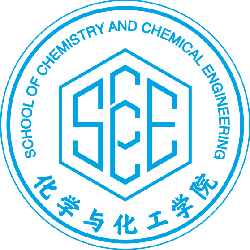
\includegraphics[width=4cm,height=4cm]{BIT-China}
}
\end{center}
\textbf{\\Team Leader}

  孙一洋


\textbf{\\Contact}

  sunyiyangvip@126.com


\textbf{\\A New Application Project\\}\begin{spacing}{1.5}

我们构建了一种以酿酒酵母为底盘细胞的生物传感器,来检测食物中的鲜甜比例及部分苦味物质。客户将通过我们的“Flavor Card”小程序,发现自己最喜爱的味道。之后我们对全价蛋白-大豆分离蛋白进行酶解,组合产生不同的风味实现私人订制。我们的酵母菌还可以对产品进行品尝,反馈给用户一个属于他们的独家色彩,是味觉与视觉的双重享受!\end{spacing}
\\

\url{https://2021.igem.org/Team:BIT-China }\\
\url{https://igem.org/Team.cgi?id=3852 }\\
\url{http://parts.igem.org/wiki/index.php?title=Part:BBa_K3852000 }\\
\url{https://video.igem.org/w/9FgKTwgLX4gD3kMoZdsu7H }\\

\vfill{}









Team of BIT-China will present between      2021/8/28 13:00-14:30   using 腾讯会议 404 469 7665.
\newpage


\subsection{\textcolor{Blu}{ BUCT-China } }
\vspace{5mm}
\begin{center}
\large{
  \textbf{ the Food of Future-Cultured Meat }\\

  
\includegraphics[width=4cm,height=4cm]{BUCT-China}
}
\end{center}
\textbf{\\Team Leader}

  张瀚艺*


\textbf{\\Contact}

  1621479460@qq.com


\textbf{\\A Food & Nutrition Project\\}\begin{spacing}{1.5}

We build three kinds of genetically engineered bacteria with reconstructed pathways to synthesize specific unsaturated fatty acid, construct new bio-material, and produce collagen. The new bio-material and collagen will be used in tissue engineering with muscle stem cell to make cultured meat.\end{spacing}
\\

\url{https://2021.igem.org/Team:BUCT-China }\\
\url{https://igem.org/Team.cgi?id=3742 }\\
\url{http://parts.igem.org/wiki/index.php?title=Part:BBa_K3742000 }\\
\url{https://video.igem.org/w/sBsvYbTeYbR7Nz9qF5M17s }\\

\vfill{}









Team of BUCT-China will present between      2021/8/28 13:00-14:30   using 腾讯会议 404 469 7665.
\newpage


\subsection{\textcolor{Blu}{ DUT\_China } }
\vspace{5mm}
\begin{center}
\large{
  \textbf{ Intricate modular enzyme assembly for enhanced PET plastic degradation and metabolic flux }\\

  
\includegraphics[width=4cm,height=4cm]{DUT_China}
}
\end{center}
\textbf{\\Team Leader}

  霍玉亮


\textbf{\\Contact}

  1589318542@qq.com

\textbf{\\An Environment Project\\}\begin{spacing}{1.5}

Wide spreading and utilization of plastic PET (polyethylene terephthalate) in the world has caused a large quantity of environmental challenges and gained much attention. In response, microbe Ideonella sakaiensis was reported to be capable of secreting two efficient enzymes to deconstruct PET polymers in environment. Hydrophobin in fungi can cupture PET and insert PET chains to divide them into partial line, which PETase can bond easily. However, this two-enzyme system degradation capacity may be highly limited due to inhibition effects and diffusion of intermediates. Therefore, we design a delicate multicomplex enzyme system, in which short peptide tags (RIAD and RIDD) are applied to create scaffold-free enzyme assemblies. Here, in order to capture and degrade microplastic PET particles effectively, we construct enzymes of PETase and MHETase and hydrophobin into our complex system, which reveal high catalytic efficiency in experiments. So we are hoping to make our efforts on the solution of plastic pollution. We plan to use E.coli and Chiamydomonas reinhardtii as chassis creature. Also, we pay more attention to biosafety in our project. We design several kill switches in the two chassis creature, to make sure their cells and modified genes will not be new threat or pollution.\end{spacing}
\\

\url{https://2021.igem.org/Team:DUT\_China }\\
\url{https://igem.org/Team.cgi?id=3898 }\\
\url{http://parts.igem.org/wiki/index.php?title=Part:BBa_K3898000 }\\
\url{https://video.igem.org/w/bgNjcwEgzp9B5t743Z4UrQ }\\

\vfill{}









Team of DUT\_China will present between   2021/8/27 17:00-18:30      using 腾讯会议 404 469 7665.
\newpage


\subsection{\textcolor{Blu}{ LZU-CHINA } }
\vspace{5mm}
\begin{center}
\large{
  \textbf{ Targeted inhibition of SARS-CoV-2 infection based on CRISPR-Cas13d system }\\

  
\includegraphics[width=4cm,height=4cm]{LZU-CHINA}
}
\end{center}
\textbf{\\Team Leader}

  朱坤


\textbf{\\Contact}

  zhuk18@lzu.edu.cn


\textbf{\\A Therapeutics Project\\}\begin{spacing}{1.5}

Currently, the world is still faced with the COVID-19 epidemic caused by novel coronavirus which urgently requires flexible and targeted protection measures. Novel coronavirus belongs to the family of forward RNA viruses. The spike proteins on its surface bind to the human cell surface receptors called ACE2 and then enter the cell through endocytosis. Reducing the expression of ACE2 does not cause significant structural abnormalities. Therefore, recognizing and inhibiting the expression level of ACE2 is considered to be an effective treatment for COVID-19. CRISPR-Cas13d is an RNA-guided ribonuclease which targets ssRNA. The RNA-targeted ribonuclease activity of Cas13d is independent of the specific adjacent sequences, which meets the requirements of rapid development of gRNA.

SARS-CoV-2 mainly infects the human respiratory and digestive systems. It causes disease through direct cytotoxic effects and inducing inflammatory response. We select human embryonic kidney cells (HEK293T), lung cells (HLF-a), colorectal cells (CCD-18Co) and gastric cells (GES-1) to establish hACE2 stable transfection lines respectively and lentivirus with novel coronavirus spike protein is used as pseudovirus. Through bioinformatics screening of crRNA pool for ACE2 conserved sequence, the lentivirus /CRISPR-Cas13d system was constructed. Specific crRNA-mediated Cas13d system is used to target and knock down the mRNA level of ACE2 in four stable cell lines, which leads to a decrease in the expression of the receptor protein ACE2 on the cell surface. Thus, entry of the pseudovirus into cells was inhibited. We will use vitro and cell experiments to verify the effect of CRISPR-Cas13d system designed by us.\end{spacing}
\\

\url{https://2021.igem.org/Team:LZU-CHINA }\\
\url{https://igem.org/Team.cgi?id=3760 }\\
\url{http://parts.igem.org/wiki/index.php?title=Part:BBa_K3760000 }\\
\url{https://video.igem.org/w/7xeCJk7DPxMERSr9z6Ftsn }\\

\vfill{}









Team of LZU-CHINA will present between    2021/8/28 8:30-10:00     using 腾讯会议 404 469 7665.
\newpage


\subsection{\textcolor{Blu}{ NAU-CHINA } }
\vspace{5mm}
\begin{center}
\large{
  \textbf{ High-efficiency selenium recovery bioreactor: engineered \textit{E. coli} }\\

  
\includegraphics[width=4cm,height=4cm]{NAU-CHINA}
}
\end{center}
\textbf{\\Team Leader}

  石国龙


\textbf{\\Contact}

  1466036548@qq.com

\textbf{\\An Environment Project\\}\begin{spacing}{1.5}

Some places are heavily polluted by selenium-oxide ions, while some places lack selenium and even suffer from it, especially in China. Selenium nanoparticles (SeNPs) are a kind of elemental selenium wrapped in biological macromolecules such as proteins. Compared with other forms of selenium, it has the advantages of low toxicity, high efficiency, smaller particle size and higher activity, and has been widely used in medicine, agriculture, animal husbandry and other aspects. Some microorganisms have the nutural ability to reduce selenium-oxide anions to SeNPs. However, they are not always perfect. There are problems such as low reduction efficiency and low activity due to large particle size of SeNPs. We chose \textit{E. coli} MG1655, which has the natural ability of reducing selenium oxide anions to SeNPs, as the chassis, added Csr F enzyme and Sef  A protein which could improve the reduction rate. Finally, a high-efficient selenium recovery bioreactor with higher reduction rate and higher product activity was obtained. The SeNPs produced in the bioreactor has been used to inhibit drug-resistant bacteria, adsorb heavy metal ions and improve the quality of crops with satisfactory results.\end{spacing}
\\

\url{https://2021.igem.org/Team:NAU-CHINA }\\
\url{https://igem.org/Team.cgi?id=3735 }\\
\url{http://parts.igem.org/wiki/index.php?title=Part:BBa_K3735000 }\\
\url{https://video.igem.org/w/8SFTfHvResh9ZR3va2AsiR }\\

\vfill{}









Team of NAU-CHINA will present between   2021/8/27 17:00-18:30      using 腾讯会议 404 469 7665.
\newpage


\subsection{\textcolor{Blu}{ OUC-China } }
\vspace{5mm}
\begin{center}
\large{
  \textbf{ ALLPASs (Amplifying Low-leakage Platform for Antibiotic Sensors) }\\

  
\includegraphics[width=4cm,height=4cm]{OUC-China}
}
\end{center}
\textbf{\\Team Leader}

  彭思源

  徐敏和

  李若萱


\textbf{\\Contact}

  oucigem@163.com

\textbf{\\An Environment Project\\}\begin{spacing}{1.5}

Due to the large-scale use of antibiotics, environmental pollution and food residues have posed a great threat to the ecological environment as well as human health. Therefore, this project aims to design a series of high-performance whole cell biosensors (WCBs) to detect antibiotics. To overcome the common limits of WCBs, a fluorescence-activated RNA aptamer is used as the output signal to increase the response speed, and it is hoped that the signal-noise ratio and dynamic range of the sensor can be improved by the NIMPLY logic gate gene circuit composed of CRISPRi and strand replacement reactions.

由于抗生素的大规模使用,其造成的环境污染和食品残留问题对生态环境与健康安全已构成了威胁,故本项目以四环素类和大环内酯类抗生素为例,设计了高性能的全细胞生物传感器用以检测抗生素。为克服全细胞生物传感器常见的各种限制,本项目将一种荧光激活RNA适配体作为输出信号以增加传感器响应速度,并希望通过由CRISPRi和链置换反应组成的NIMPLY逻辑门基因线路提高传感器的信噪比 (signal-noise ratio) 和动态范围。\end{spacing}
\\

\url{https://2021.igem.org/Team:OUC-China }\\
\url{https://igem.org/Team.cgi?id=3777 }\\
\url{http://parts.igem.org/wiki/index.php?title=Part:BBa_K3777000 }\\
\url{https://video.igem.org/w/eH2fZPe25RCARXWrH8zW7i }\\

\vfill{}









Team of OUC-China will present between   2021/8/27 17:00-18:30      using 腾讯会议 404 469 7665.
\newpage


\subsection{\textcolor{Blu}{ ShanghaiTech\_China } }
\vspace{5mm}
\begin{center}
\large{
  \textbf{ Mussel Inspired Biologically Operational Material (MIBOM) }\\

  
\includegraphics[width=4cm,height=4cm]{ShanghaiTech_China}
}
\end{center}
\textbf{\\Team Leader}

  苏睿


\textbf{\\Contact}

  352373393@qq.com


\textbf{\\A New Application Project\\}\begin{spacing}{1.5}

MIBOM全称为“Mussel Inspired Biologically Operational Material”,是以贻贝粘蛋白为核心,结合新材料与细胞工程开发的全新一代生物材料。目前项目已相对成熟地开发了新一代的骨修复凝胶,用于治疗粉碎性骨折。团队开发了独创的“贻贝粘蛋白+水凝胶+细胞工程”模块化开发思路,为多种产品的开发创生了高效率、低成本的研发潜力。

MIBOM团队一直关注利用合成生物学、新材料等前沿技术来实现可持续发展。产品目前已经过多次迭代,引入了粘附、调控、给药、凝胶系统,并且在硬件上加载光固化系统,完成了总体应用场景的设计。我们同时设计了与MIBOM产品相应的模块化产品,引入“贻贝粘蛋白+功能化水凝胶+功能化细胞调控通路”作为模块产品的核心设计,用于在未来开展面向其他领域的研发。\end{spacing}
\\

\url{https://2021.igem.org/Team:ShanghaiTech\_China }\\
\url{https://igem.org/Team.cgi?id=3755 }\\
\url{http://parts.igem.org/wiki/index.php?title=Part:BBa_K3755000 }\\
\url{https://video.igem.org/w/oBWPv3ZEZGkXiGfdwzXMpR }\\

\vfill{}









Team of ShanghaiTech\_China will present between      2021/8/28 13:00-14:30   using 腾讯会议 404 469 7665.
\newpage


\subsection{\textcolor{Blu}{ SUSTech\_Shenzhen } }
\vspace{5mm}
\begin{center}
\large{
  \textbf{ 开发可防止腹泻脱水的肠道工程菌 Development of gut microbes to prevent diarrhea-related dehydration }\\

  
\includegraphics[width=4cm,height=4cm]{SUSTech_Shenzhen}
}
\end{center}
\textbf{\\Team Leader}

  龚颖璇

  屈泽阳


\textbf{\\Contact}

  11911518@mail.sustech.edu.cn


\textbf{\\A Therapeutics Project\\}\begin{spacing}{1.5}

脱水是导致腹泻相关死亡的主要原因之一,因此我们计划设计一种可以帮助腹泻患者保持水分并且杀灭病原菌的有益工程微生物,通过在细菌中合成colanic acid,实现对于水分的存储。在第一阶段的研究中,我们希望通过开发一种工程微生物来治疗霍乱,这种由霍乱弧菌导致的严重疾病。霍乱的主要症状是十分严重的脱水,如果不加以治疗,患者可能在短短几个小时内失去生命。鉴于合成生物学的模块化特性,在后续的研究中,不同种类的工程微生物将会被设计,以抵御不同的病原体。通过宿主的脱水的症状以及霍乱弧菌的触发的colanic acid的生物合成来调节水储存,以保持宿主的水分。这种脱水信号包括感应肠道氯浓度的升高和霍乱弧菌群体感应分子。同时,这些信号还会促进广谱抗菌肽(AMPs)的触发释放,以消灭引起腹泻的肠道病原体。该设计旨在创造一种低成本、易于获取和方便的腹泻治疗方法。\end{spacing}
\\

\url{https://2021.igem.org/Team:SUSTech\_Shenzhen }\\
\url{https://igem.org/Team.cgi?id=3914 }\\
\url{http://parts.igem.org/wiki/index.php?title=Part:BBa_K3914000 }\\
\url{https://video.igem.org/w/4Khi8unRKGKcFQg3L4ShNL }\\

\vfill{}









Team of SUSTech\_Shenzhen will present between    2021/8/28 8:30-10:00     using 腾讯会议 404 469 7665.
\newpage


\subsection{\textcolor{Blu}{ SZPT-CHINA } }
\vspace{5mm}
\begin{center}
\large{
  \textbf{ Kissed by Light }\\

  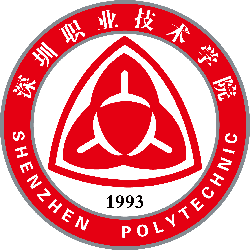
\includegraphics[width=4cm,height=4cm]{SZPT-CHINA}
}
\end{center}
\textbf{\\Team Leader}

  刘婉婷


\textbf{\\Contact}

  SZPTCHINA2021@163.com


\textbf{\\A Therapeutics Project\\}\begin{spacing}{1.5}

Infection remains the most common cause of morbidity and mortality in burn patients. \textit{Pseudomonas aeruginosa} is among the leading causes of nosocomial infection primarily because it is intrinsically resistant to many antibiotics and antimicrobials.

This year our team is working on \textit{P. aeruginosa} infection and wound repair in burn treatment. Using principles of synthetic biology, we genetically modified \textit{Gluconacetobacter xylinus} ATCC53582 to kill \textit{P. aeruginosa} specifically through the production and release of chimeric bacteriocin SE protein and the immune protein. Moreover, the production of cellulose in the engineered \textit{Gluconacetobacter xylinus} ATCC53582 was regulated by blue light,which can further prevent infection of other bacteria and promote wound repair.\end{spacing}
\\

\url{https://2021.igem.org/Team:SZPT-CHINA }\\
\url{https://igem.org/Team.cgi?id=3740 }\\
\url{http://parts.igem.org/wiki/index.php?title=Part:BBa_K3740000 }\\
\url{https://video.igem.org/w/4mCGZkJCF2ZDwC5d4zZq5q }\\

\vfill{}









Team of SZPT-CHINA will present between    2021/8/28 8:30-10:00     using 腾讯会议 404 469 7665.
\newpage


\subsection{\textcolor{Blu}{ Tianjin } }
\vspace{5mm}
\begin{center}
\large{
  \textbf{ CREATE: Chromosome Released Eukaryocyte which is Active, Transitory and Environment-friendly }\\

  
\includegraphics[width=4cm,height=4cm]{Tianjin}
}
\end{center}
\textbf{\\Team Leader}

  丁泠薇


\textbf{\\Contact}

  2429736514@qq.com


\textbf{\\A Foundational Advance Project\\}\begin{spacing}{1.5}

Tianjin team demonstrated CREATE, a kind of eukaryotic cell that removes chromosomes. As it gets rid of the chromosomes, it has other functions, such as good biological safety. Thus, it can be applied to drug delivery and large DNA fragments transfer and other aspects.

Tianjin团队突破自然桎梏,设计了一种无染色体酵母,无染色体的条件赋予了细胞不繁殖却有活性的特殊性质,在多方面具有极大应用潜力。\end{spacing}
\\

\url{https://2021.igem.org/Team:Tianjin }\\
\url{https://igem.org/Team.cgi?id=3939 }\\
\url{http://parts.igem.org/wiki/index.php?title=Part:BBa_K3939000 }\\
\url{https://video.igem.org/w/fBhJRd7irTLZTm7BPynGak }\\

\vfill{}









Team of Tianjin will present between     2021/8/28 10:30-12:00    using 腾讯会议 404 469 7665.
\newpage


\subsection{\textcolor{Blu}{ UCAS-China } }
\vspace{5mm}
\begin{center}
\large{
  \textbf{ DeCaffi }\\

  
\includegraphics[width=4cm,height=4cm]{UCAS-China}
}
\end{center}
\textbf{\\Team Leader}

  陈冠羽

  刘启涵*


\textbf{\\Contact}

  C867469688@hotmail.com


\textbf{\\A Food & Nutrition Project\\}\begin{spacing}{1.5}

Our project aims to remove caffeine from drinks by synthetic biology methods. To achieve this goal, we will convert caffeine into healthful theacrine through a two-step enzymatic reaction in a cell-free system. This process requires two enzymes: Cdh and CkTcS, which will be produced by our engineered bacteria modified by synthetic biology methods These two enzymes can utilize CoQ(0) and SAM to turn caffeine into theacrine. For this aim, we will also use engineered bacteria for fermentatve production of SAM. In addition, we I use the PUTR-CRP global transcrptional regulatory system to enhance the expression of target genes. All our genetically modified engineered bacteria will be strictly confined to the laboratory culture, and we will also transfer the cryo-induced suicide module relB-relE+Ptrc into them to eliminate the risk of engineered bacteria's leaking. Finally, all substances needed in the decaffeine process will be purified, sterilized and then added to the cartridges. Through this. we can ensure that our cartridges can be used to filter drinks without causing harm to humans and the environment.\end{spacing}
\\

\url{https://2021.igem.org/Team:UCAS-China }\\
\url{https://igem.org/Team.cgi?id=3817 }\\
\url{http://parts.igem.org/wiki/index.php?title=Part:BBa_K3817000 }\\
\url{https://video.igem.org/w/92VHYCZ9cXW21a4JfhS9wY }\\

\vfill{}









Team of UCAS-China will present between      2021/8/28 13:00-14:30   using 腾讯会议 404 469 7665.
\newpage


\subsection{\textcolor{Blu}{ USTC-Software } }
\vspace{5mm}
\begin{center}
\large{
  \textbf{ CAT: Convenient, Accurate Tool }\\

  
\includegraphics[width=4cm,height=4cm]{USTC-Software}
}
\end{center}
\textbf{\\Team Leader}

  沈蜀媛


\textbf{\\Contact}

  sue@mail.ustc.edu.cn


\textbf{\\A Software Project\\}\begin{spacing}{1.5}

Nowadays, machine learning has been devoted to various areas, and has made some magnificent contribution in Synthetic biology, for example, Alphafold2 by Google, which can accurately predict the 3D structure by protein sequence, and some other models predicting the properties of protein sequence. But recently there is still lack of tools that is user-friendly and can integrate existing model and software. Thus, CAT, Convenient Accurate Tool, is designed. Based on the purpose of offering an highly-efficient software to our user, we collect some important properties of protein sequence. Moreover, we combine CAT with education and build up a education version in order to briefly introduce the models and the achievement that machine learning has done in synthetic biology. By the education version, we hope that CAT can motivate students' interest and make further contribution in the area of synthetic biology and machine learning.

如今机器学习在各个领域都有着显著的成果,并且在合成生物学领域也做出了极大的贡献,例如能精准预测蛋白质三级结构的Alphafold2。但是现在还缺乏一个用户友好且将这些模型整合在一起的工具,CAT由此诞生了,我们集结一些重要的属性预测,使用户能高效的得到想要的结果,并且结合教育,搭建一个教育版,介绍所用模型以及应用在合成生物学中的成果。\end{spacing}
\\

\url{https://2021.igem.org/Team:USTC-Software }\\
\url{https://igem.org/Team.cgi?id=3958 }\\
\url{http://parts.igem.org/wiki/index.php?title=Part:BBa_K3958000 }\\
\url{https://video.igem.org/w/vNGx3WsXWis16YcqSDY3yB }\\

\vfill{}









Team of USTC-Software will present between 2021/8/27 13:00-14:30        using 腾讯会议 404 469 7665.
\newpage


\subsection{\textcolor{Blu}{ ZJUT-China } }
\vspace{5mm}
\begin{center}
\large{
  \textbf{ CRISPR/Cas9-based Cell-Free Biosensors For RNA Biomarkers }\\

  
\includegraphics[width=4cm,height=4cm]{ZJUT-China}
}
\end{center}
\textbf{\\Team Leader}

  王晓祺


\textbf{\\Contact}

  262758046@qq.com


\textbf{\\A New Application Project\\}\begin{spacing}{1.5}

According to literature, various RNA molecules in urine or blood have proven to serve as biomarkers for the diagnosis and prognosis of various diseases. Herein, we are developing a cell-free RNA biosensor, which comprises a cell-free system, engineered DNA transcription templates and RNA-responsive CRISPR/Cas9 System. We hope our project will provide patients with a simple, safe, low-cost diagnostic method.\end{spacing}
\\

\url{https://2021.igem.org/Team:ZJUT-China }\\
\url{https://igem.org/Team.cgi?id=3885 }\\
\url{http://parts.igem.org/wiki/index.php?title=Part:BBa_K3885000 }\\
\url{https://video.igem.org/w/qgfpuHjrEcw1JgiY8o75y8 }\\

\vfill{}









Team of ZJUT-China will present between       2021/8/28 15:00-16:30  using 腾讯会议 404 469 7665.
\newpage


\subsection{\textcolor{Blu}{ FZU-China } }
\vspace{5mm}
\begin{center}
\large{
  \textbf{ Development of optogenetic switch-based gut bacteria to potentially alleviate depression by supplementing GABA }\\

  
\includegraphics[width=4cm,height=4cm]{FZU-China}
}
\end{center}
\textbf{\\Team Leader}

  张慧敏


\textbf{\\Contact}

  1290703830@qq.com


\textbf{\\A Therapeutics Project\\}\begin{spacing}{1.5}

We design a biocircuit with four different modules: a light module, an optogenetic switch module, a GABA module, and a lysis module. The light module contains light-generating genes luxCDABE under the control of a T7 promoter and a lac operator. The optogenetic switch module contains a light-switchable domain VVD and a split recombinase Cre under the control of a pLac promoter. The GABA module and lysis module contain a GABA-producing enzyme gadB and a lysis protein φX174E under the control of a PW4 promoter and a LoxP-terminator-LoxP fragment. LuxAB is a luciferase which can utilize the aldehyde made by LuxCDE to produce blue-green light. When exposed to blue light, VVDs change conformation to allow dimerization, which brings the Cre fragments together to make it an active recombinase. Cre recombinase then recognize and excise DNA fragments flanked by two loxP sites. The excision eliminates the terminator placed 3' of the promoter, so the following genes can be transcribed and translated into GadB and φX174E proteins. GadB catalyzes the conversion of glutamate to GABA. φX174E induces cell wall lysis to release intracellular GABAs into human gut environment.\end{spacing}
\\

\url{https://2021.igem.org/Team:FZU-China }\\
\url{https://igem.org/Team.cgi?id=3769 }\\
\url{http://parts.igem.org/wiki/index.php?title=Part:BBa_K3769000 }\\


\vfill{}









Team of FZU-China will present between    2021/8/28 8:30-10:00     using 腾讯会议 404 469 7665.
\newpage


\subsection{\textcolor{Blu}{ SCAU-China } }
\vspace{5mm}
\begin{center}
\large{
  \textbf{ MESEG (metal eater-super environmental guard) }\\

  
\includegraphics[width=4cm,height=4cm]{SCAU-China}
}
\end{center}
\textbf{\\Team Leader}

  梁经伦


\textbf{\\Contact}

  scauchina2021@163.com

\textbf{\\An Environment Project\\}\begin{spacing}{1.5}

水体重金属污染问题不可小觑,本项目利用莱茵衣藻的自噬途径并在基因层面加以改造,将重金属结合蛋白与自噬相关蛋白在莱茵衣藻中融合表达,使其吸收水体中的重金属并存储到液泡中,通过集中打捞来回收水体中的重金属。为防止基因泄露,设计了固定装置,辅以海藻酸钠包埋法包裹莱茵衣藻,为其提供稳定的生长环境,同时有助于回收打捞。\end{spacing}
\\

\url{https://2021.igem.org/Team:SCAU-China }\\
\url{https://igem.org/Team.cgi?id=4014 }\\
\url{http://parts.igem.org/wiki/index.php?title=Part:BBa_K4014000 }\\
\url{https://video.igem.org/w/nXN6WCWKNXkm1Yaf1VeQJ3 }\\

\vfill{}









Team of SCAU-China will present between   2021/8/27 17:00-18:30      using 腾讯会议 404 469 7665.
\newpage


\subsection{\textcolor{Blu}{ WHU-China } }
\vspace{5mm}
\begin{center}
\large{
  \textbf{ Acneraser }\\

  
\includegraphics[width=4cm,height=4cm]{WHU-China}
}
\end{center}
\textbf{\\Team Leader}

  毛丽然


\textbf{\\Contact}

  1299815609@qq.com


\textbf{\\A Therapeutics Project\\}\begin{spacing}{1.5}

Acne is a common skin disease. Generally speaking, acne is related to pores being blocked by sebum and propionibacterium acnes proliferating in such an anaerobic environment. Our project aims at acne caused by such factors and hopes to develop a drug for acne treatment with less side effects and convenience. On the one hand, our engineering bacteria have stronger ability to break down fatty acids, unblocking the pores, which will destroy the anaerobic environment. On the other hand, our engineering bacteria can secrete bacteriocin which is able to kill propionibacterium acnes. At the same time, in order to ensure the precise synthesis and secretion of killing substances, we added fatty acid-sensitive promoters before bacteriocin. We hope to further optimize the function of the promoters by means of directed evolution. In terms of safety, we will prevent environmental pollution or other safety threats by using nutritionally deficient engineered bacteria.\end{spacing}
\\

\url{https://2021.igem.org/Team:WHU-China }\\
\url{https://igem.org/Team.cgi?id=3763 }\\
\url{http://parts.igem.org/wiki/index.php?title=Part:BBa_K3763000 }\\
\url{https://video.igem.org/w/89LTifDbpfJ6S2sYpXxNzc }\\

\vfill{}









Team of WHU-China will present between    2021/8/28 8:30-10:00     using 腾讯会议 404 469 7665.
\newpage


\subsection{\textcolor{Blu}{ HUST-China } }
\vspace{5mm}
\begin{center}
\large{
  \textbf{ Mr. Tony }\\

  
\includegraphics[width=4cm,height=4cm]{HUST-China}
}
\end{center}
\textbf{\\Team Leader}

  樊昌鑫

  石家诚

  王博涵


\textbf{\\Contact}

  867834428@qq.com


\textbf{\\A Manufacturing Project\\}\begin{spacing}{1.5}

Our project is about an engineering yeast which can secrete peptides and/or pigments to perm and dye people's hair without harm and it can also straight hair and decompose pigments. We also design a device and hair creams to use at daily lives. We hope our products can fly people's dreams which to pursuit beauty and make the elderly to color their hair without worries.\end{spacing}
\\

\url{https://2021.igem.org/Team:HUST-China }\\
\url{https://igem.org/Team.cgi?id=3711 }\\
\url{http://parts.igem.org/wiki/index.php?title=Part:BBa_K3711000 }\\
\url{https://video.igem.org/w/aMwNT6eBryGs8xG5avXD51 }\\

\vfill{}









Team of HUST-China will present between 2021/8/27 13:00-14:30        using 腾讯会议 404 469 7665.
\newpage


\subsection{\textcolor{Blu}{ HUST2-China } }
\vspace{5mm}
\begin{center}
\large{
  \textbf{ NANOCleaner }\\

  
\includegraphics[width=4cm,height=4cm]{HUST2-China}
}
\end{center}
\textbf{\\Team Leader}

  李一凡


\textbf{\\Contact}

  1195626066@qq.com


\textbf{\\A Diagnostics Project\\}\begin{spacing}{1.5}

In 2010, acne was the eighth epidemic, accounting for 9.38\% of the global population. From 2006 to 2016, the global prevalence of acne increased by 5.1\%. The human body's innate immunity and inflammation of P. acnes is the key to acne pathology and sequelae. Therefore, we designed an engineered bacteria that can bind to the base of the mask express two fusion proteins under infrared-induced condition. The two fusion proteins can be aggregated into nanospheres to achieve killing and blocking of \textit{Propionibacterium acnes}. Inflammation can achieve the purpose of curing acne and repairing the skin. We have successfully expressed our proteins and achieved temperature-controlled self-aggregation \textit{in vitro}.\end{spacing}
\\

\url{https://2021.igem.org/Team:HUST2-China }\\
\url{https://igem.org/Team.cgi?id=3712 }\\
\url{http://parts.igem.org/wiki/index.php?title=Part:BBa_K3712000 }\\
\url{https://video.igem.org/w/mgpajRJyEGsVQnDwtuHudc }\\

\vfill{}









Team of HUST2-China will present between        2021/8/28 17:00-18:30 using 腾讯会议 404 469 7665.
\newpage


\subsection{\textcolor{Blu}{ LZU-HS-CHINA } }
\vspace{5mm}
\begin{center}
\large{
  \textbf{ NANO'S Eagerness, Probiotics Synthesis of SeNPs }\\

  
\includegraphics[width=4cm,height=4cm]{LZU-HS-CHINA}
}
\end{center}
\textbf{\\Team Leader}

  刘觐荣


\textbf{\\Contact}

  1746921258@qq.com


\textbf{\\A High-School Food & Nutrition Project\\}\begin{spacing}{1.5}

Selenium plays an important role in balancing the systems in human bodies and sustaining the stability of human organs. Selenium deficiency would cause severe diseases like Keshan diseases, Cataracts, Diabetes, and other organic diseases in body systems.

Selenium deficiency is prevailing globally. Moreover, China is one of the countries that has tens of thousands of people suffer from its relevant diseases because nearly 72 percent of the land are lack of selenium supply to the crops and livestock while eating is the primary approach of absorbing Se.

Solutions are not efficacious and advantageous enough and problems remain. The common selenium supplements cure only the symptoms, and the supplements can seldom control the amount absorb by body, which will cause selenosis if over-ingestion take place. Besides, synthesizing selenium in chemical media has a low output capacity, producing toxic by-products that might contaminate the environment and threaten the health of human bodies.

With our discovery of Staphylococcus aureus LZ-01, a special bacteria that act as an enhancer for the production of SeNPs supplements, the output capacity of SeNPs will dramatically increase and the synthesis will no longer rely on poisonous and unstable chemical and physical conditions.\end{spacing}
\\

\url{https://2021.igem.org/Team:LZU-HS-CHINA }\\
\url{https://igem.org/Team.cgi?id=3986 }\\
\url{http://parts.igem.org/wiki/index.php?title=Part:BBa_K3986000 }\\
\url{https://video.igem.org/w/ihwMoyxfUSQXyM8dB2wVeU }\\

\vfill{}









Team of LZU-HS-CHINA will present between       2021/8/28 15:00-16:30  using 腾讯会议 404 469 7665.
\newpage


\subsection{\textcolor{Blu}{ Think\_Edu\_China } }
\vspace{5mm}
\begin{center}
\large{
  \textbf{ DEBIOTICS — Degradation of Antibiotics }\\

  
\includegraphics[width=4cm,height=4cm]{Think_Edu_China}
}
\end{center}
\textbf{\\Team Leader}

  刘觐荣


\textbf{\\Contact}

  1746921258@qq.com


\textbf{\\A High-School Environment Project\\}\begin{spacing}{1.5}

Antibiotics, which served as an agent that can kill the bacteria effectively, plays a crucial role in treating and preventing bacterial infection. However, it was abused in many fields, especially animal husbandry. Over the recent years, the use of antibiotics has caused heated debate and controversy. Meanwhile, the degradation efficiency of antibiotics has not kept pace with their wide range of animal hunsbandry applications. Scientists hypothesized that the consumption of antibiotics in edible animal will surge from 23\% in 2010 to 30\% in 2030. The harm of adding antibiotics in feed is mainly reflected in two aspects: the accumulation in poultries, and the increasing in the resistance of bacteria, which may lead to the form of super-bacteria that could be detrimental to both environment and living beings.

While, Conventional methods like high temperature composting, fermentation and microbial degradation have some potential problems including low efficiency and high costs. Effective new methods are urgently needed.

Fortunately, the Whole Cell Biocatalyst Ecn-IL, can be a favorable solution to the mentioned issue. With the technology of cell surface display, the \textit{Laccase} gene (lacc6) which originated from \textit{Pleurotus ostreatus} can be displayed on the surface of Probiotic \textit{E. coli}, Nissle 1917 (EcN), and form a membrane-like mechanism to decompose the antibiotics residues. The utilization of the Ecn-Il can effectively avoid the accumulation of the antibiotics in animals. Besides, without the mountainous usages of antibiotics, the tolerability can be largely reduced, and thus the formation of the super-bacteria can also be avoided. More importantly, the Ecn-IL is friendly to the environment. Specifically, when using the Ecn-IL, people can save much resources and eliminate the residual of the antibiotics that lie in the waste-water, soil, and animals' excrement at the same time.\end{spacing}
\\

\url{https://2021.igem.org/Team:Think\_Edu\_China }\\
\url{https://igem.org/Team.cgi?id=3984 }\\
\url{http://parts.igem.org/wiki/index.php?title=Part:BBa_K3984000 }\\
\url{https://video.igem.org/w/m84UzewU64GfTb2Ww2p7h9 }\\

\vfill{}









Team of Think\_Edu\_China will present between   2021/8/27 17:00-18:30      using 腾讯会议 404 469 7665.
\newpage


\subsection{\textcolor{Blu}{ XHD-Wuhan-Pro-China } }
\vspace{5mm}
\begin{center}
\large{
  \textbf{ 漆酶 }\\

  
\includegraphics[width=4cm,height=4cm]{XHD-Wuhan-Pro-China}
}
\end{center}
\textbf{\\Team Leader}

  刘觐荣


\textbf{\\Contact}

  1746921258@qq.com


\textbf{\\A High-School Project\\}\begin{spacing}{1.5}

No abstract submited before Aug 24th 2021.\end{spacing}
\\

\url{https://2021.igem.org/Team:XHD-Wuhan-Pro-China }\\
\url{https://igem.org/Team.cgi?id=3925 }\\
\url{http://parts.igem.org/wiki/index.php?title=Part:BBa_K3925000 }\\


\vfill{}









Team of XHD-Wuhan-Pro-China will present between  2021/8/27 15:00-16:30       using 腾讯会议 404 469 7665.
\newpage


\subsection{\textcolor{Blu}{ ECUST\_China } }
\vspace{5mm}
\begin{center}
\large{
  \textbf{ Magic Blue }\\

  
\includegraphics[width=4cm,height=4cm]{ECUST_China}
}
\end{center}
\textbf{\\Team Leader}

  陆宇晴


\textbf{\\Contact}

  2431056766@qq.com


\textbf{\\A Food & Nutrition Project\\}\begin{spacing}{1.5}

We are the 2021 iGEM team,Magic Blue. As shown by our name,we hope to get a kind of healthy blue pigment—phycocyanin,letting more people have the taste of blue. Using yeast as the carrier, it's safe and convenient to access to food. The brief process is that we insert two modified plasmids into it, finally generates phycocyanin in the cytosol, making the yeast appear blue.\end{spacing}
\\

\url{https://2021.igem.org/Team:ECUST\_China }\\
\url{https://igem.org/Team.cgi?id=3970 }\\
\url{http://parts.igem.org/wiki/index.php?title=Part:BBa_K3970000 }\\
\url{https://video.igem.org/w/nMCYSPcaEtS4CFKLZNmVsb }\\

\vfill{}









Team of ECUST\_China will present between      2021/8/28 13:00-14:30   using 腾讯会议 404 469 7665.
\newpage


\subsection{\textcolor{Blu}{ GreatBay\_SCIE } }
\vspace{5mm}
\begin{center}
\large{
  \textbf{ ONCOKILLER: Aptamer functionalized drugs for the curing of HER2 positive breast cancer }\\

  \includegraphics[width=4cm,height=4cm]{GreatBay_SCIE}
}
\end{center}
\textbf{\\Team Leader}

  李彦喆*

  赵若朴


\textbf{\\Contact}

  scie\_igem@outlook.com


\textbf{\\A High-School Therapeutics Project\\}\begin{spacing}{1.5}

Our project aims at utilizing aptamers and nanoparticles to develop a new type of breast cancer targeting-drugs. Using aptamers as guide molecules can provide us with advantages such as lower production costs and shorter production period; nanoparticles can increase the stability of our drug delivery system and reduce its cytotoxicity.\end{spacing}
\\

\url{https://2021.igem.org/Team:GreatBay\_SCIE }\\
\url{https://igem.org/Team.cgi?id=3897 }\\
\url{http://parts.igem.org/wiki/index.php?title=Part:BBa_K3897000 }\\
\url{https://video.igem.org/w/iv6QEJPGcCw15eHvxpd7mL }\\

\vfill{}









Team of GreatBay\_SCIE will present between     2021/8/28 10:30-12:00    using 腾讯会议 404 469 7665.
\newpage


\subsection{\textcolor{Blu}{ Tsinghua } }
\vspace{5mm}
\begin{center}
\large{
  \textbf{ IBD的益生菌联合疗法与新型诊断工具 }\\

  \includegraphics[width=4cm,height=4cm]{Tsinghua}
}
\end{center}
\textbf{\\Contact}

  jeremyliu755@foxmail.com


\textbf{\\A Therapeutics Project\\}\begin{spacing}{1.5}

炎症性肠病 (IBD) 是一类慢性肠道疾病,具有发病机理不明、检测金标准尚无且极难治愈的特点。Tsinghua iGEM 2021 团队旨在开发一种IBD的综合诊断治疗模式,从发病根源处减轻IBD症状。

为此,我们从代谢、肠道菌群和免疫调节三个角度分别设计了工程肠道益生菌,对炎症部位进行原位治疗。通过开发基于 miRNA 检测的 PLCIRT 系统,我们努力探索IBD诊断的新范式。\end{spacing}
\\

\url{https://2021.igem.org/Team:Tsinghua }\\
\url{https://igem.org/Team.cgi?id=3924 }\\
\url{http://parts.igem.org/wiki/index.php?title=Part:BBa_K3924000 }\\


\vfill{}









Team of Tsinghua will present between     2021/8/28 10:30-12:00    using 腾讯会议 404 469 7665.
\newpage


\subsection{\textcolor{Blu}{ BIT } }
\vspace{5mm}
\begin{center}
\large{
  \textbf{ ESC: Early Secondary Screening of Colorectal Cancer }\\

  \includegraphics[width=4cm,height=4cm]{BIT}
}
\end{center}
\textbf{\\Team Leader}

  刘周密*

  叶子帆

  严梓涵

  周泰言


\textbf{\\Contact}

  870912295@qq.com


\textbf{\\A Diagnostics Project\\}\begin{spacing}{1.5}

项目致力于开发的肠早康——结直肠癌辅助早筛系统,以实现在健康人群中辅助早筛结直肠癌患者和实现临床结直肠镜不耐受患者的辅助诊疗为根本目标,以生物传感体系结合自滑动芯片与配套仪器设备为技术手段,以实现准确、快速、高通量、低成本与自动一体化的检测为基本要求,最终实现易操作与结果可视化的商用化检测设备。\end{spacing}
\\

\url{https://2021.igem.org/Team:BIT }\\
\url{https://igem.org/Team.cgi?id=3821 }\\
\url{http://parts.igem.org/wiki/index.php?title=Part:BBa_K3821000 }\\
\url{https://video.igem.org/w/iMMCBzkN2KVbRgUmix4Pm6 }\\

\vfill{}









Team of BIT will present between        2021/8/28 17:00-18:30 using 腾讯会议 404 469 7665.
\newpage


\subsection{\textcolor{Blu}{ BNUZ-China } }
\vspace{5mm}
\begin{center}
\large{
  \textbf{ \textit{E. coli} Keen Doctor }\\

  \includegraphics[width=4cm,height=4cm]{BNUZ-China}
}
\end{center}
\textbf{\\Team Leader}

  杜芸希

  刘路旋


\textbf{\\Contact}

  luxuan.liu6@mail.bnu.edu.cn


\textbf{\\A Therapeutics Project\\}\begin{spacing}{1.5}

慢性肾病 (CKD) 是一种发病率高、预后差、并发症复杂的重大慢性疾病,对人类健康造成极大危害。在CKD的发生发展过程中,患者常常出现肠道菌群及其代谢紊乱、肠道屏障功能受损等现象。因此,BNUZ-China团队拟以大肠杆菌 Nissle 1917 为基盘生物,开发一种新型肠道工程菌,使工程菌具有消除肠源内毒素,调节肠道菌群结构,修复肠粘膜屏障的功能,达到治疗慢性肾病的目的。\end{spacing}
\\

\url{https://2021.igem.org/Team:BNUZ-China }\\
\url{https://igem.org/Team.cgi?id=3784 }\\
\url{http://parts.igem.org/wiki/index.php?title=Part:BBa_K3784000 }\\


\vfill{}









Team of BNUZ-China will present between     2021/8/28 10:30-12:00    using 腾讯会议 404 469 7665.
\newpage


\subsection{\textcolor{Blu}{ CHINA-FAFU } }
\vspace{5mm}
\begin{center}
\large{
  \textbf{ Microscopic Algae, Macroscopic Energy }\\

  \includegraphics[width=4cm,height=4cm]{CHINA-FAFU}
}
\end{center}
\textbf{\\Team Leader}

  殷炜铧

  董广辉


\textbf{\\Contact}

  weihua\_yinforworking@foxmail.com


An Energy Project\\}\begin{spacing}{1.5}

Microalgae, as one of the photosynthetic organisms with high carbon sequestration efficiency, have become a promising research area to achieve the goal of “carbon peaking and carbon neutrality”. The team took the common single-cell oil-producing diatom Trionyxus triangularis as the starting point, and used synthetic biology, molecular biology, bioinformatics, biochemistry, pharmacology, metabolomics, transcriptomics, etc. to explore the connection between microalgae oil synthesis and related key genes, based on which the engineered microalgae were constructed. At the same time, the completed strains will be combined with laboratory results for modeling and further screening of engineered microalgae suitable for large-scale plant applications. The research results obtained by the team will actively and effectively provide a new impetus to combat climate change, energy shortage and green low-carbon development. In addition, together with domestic and international experts, scholars and entrepreneurs in the same field, we will promote the achievement of China's and global carbon peak and carbon neutral goals.\end{spacing}
\\

\url{https://2021.igem.org/Team:CHINA-FAFU }\\
\url{https://igem.org/Team.cgi?id=3812 }\\
\url{http://parts.igem.org/wiki/index.php?title=Part:BBa_K3812000 }\\
\url{https://video.igem.org/w/n8CAF5Nc1sMFx1uKU4Eoyh }\\

\vfill{}









Team of CHINA-FAFU will present between  2021/8/27 15:00-16:30       using 腾讯会议 404 469 7665.
\newpage


\subsection{\textcolor{Blu}{ ED-NAU } }
\vspace{5mm}
\begin{center}
\large{
  \textbf{ Directed evolution of OsNramp5 in yeast }\\

  \includegraphics[width=4cm,height=4cm]{ED-NAU}
}
\end{center}
\textbf{\\Team Leader}

  郑奕彤


\textbf{\\Contact}

  10118219@njau.edu.cn


\textbf{\\A Food & Nutrition Project\\}\begin{spacing}{1.5}

Rice is an important food crop in the world.  For a long time, excessive cadmium in rice has seriously affected the grain yield and human health.  OsNramp5 is the main absorption channel of Mn2+ and Cd2+ in rice roots.  Current modification on OsNramp5 managed to reduce the absorption of Cd2+, at the cost of lack of Mn2+, resulting in rice yield reduction.  Therefore, we tried to obtain a mutant through directed evolution, which could achieve low Cd2+ absorption and at the same time meet the normal requirements of rice for Mn2+.  We constructed OsNramp5 mutant library by error-prone PCR and we respectively performed high-throughput screening in yeast using cadmium probe and manganese probe.  After preliminary screening and sequencing, coupled with site-directed mutagenesis, we expect to achieve the accumulation and iteration of favorable mutations.  We hope that the evolved mutant protein can be used in the cultivation of low-cadmium rice to produce a healthy crop.\end{spacing}
\\

\vfill{}









Team of ED-NAU will present between      2021/8/28 13:00-14:30   using 腾讯会议 404 469 7665.
\newpage


\subsection{\textcolor{Blu}{ HiZJU-China } }
\vspace{5mm}
\begin{center}
\large{
  \textbf{ EE2limination }\\

  \includegraphics[width=4cm,height=4cm]{HiZJU-China}
}
\end{center}
\textbf{\\Team Leader}

  贾思宁


\textbf{\\Contact}

  599869193@qq.com

\textbf{\\An Environment Project\\}\begin{spacing}{1.5}

17 α-ethynyl estradiol (EE2) is an artificial estrogen with a strong estrogenic effect.

The main component of contraceptives, EE2, will cause some serious diseases after intake. Because of no effective degradation method, estrogens are still accumulating in the environment. Therefore, HI-ZJU team decided to solve EE2 pollution problem. We obtained two target genes, amoA and hao, which can degrade EE2 by the way of co-metabolism, from ammonia oxidizing bacteria. Using these genes, we are able to create bacteria that can degrade EE2 by gene editing. Meanwhile, hold a pragmatic standpoint of our wastewater treatment practice (WWTP), we managed to making acquaintance with the local authority in charge of waste water recycling. Staff there introduce us to develop a treatment with high-sensibility of detecting the soluble 17 α-ethynyl estradiol in natural condition, whose percentage composition present to be relevantly low in order of magnitudes. Taking low level of EE2‘s background concentration in consideration, we managed to develop an effective and synthetic biological cascade amplification reaction superior to its rudimental form, which is competent to capture the EE2 via hydrophobic interaction between amino acid residue. We employ the artificial intelligence, a series of programs modified to bring upon hybrid on mutant site and calculate the combining Gibbs Free energy to sort out the best choice. In addition we attach a visible measurement he Green fluorescent protein (GFP), to the expression sequence of plasmid, which can linear indicates the content of EE2 in waste water.\end{spacing}
\\

\url{https://2021.igem.org/Team:HiZJU-China }\\
\url{https://igem.org/Team.cgi?id=3978 }\\
\url{http://parts.igem.org/wiki/index.php?title=Part:BBa_K3978000 }\\


\vfill{}









Team of HiZJU-China will present between   2021/8/27 17:00-18:30      using 腾讯会议 404 469 7665.
\newpage


\subsection{\textcolor{Blu}{ HZAU-China } }
\vspace{5mm}
\begin{center}
\large{
  \textbf{ P.E.T: Pets' Enteric Test }\\

  \includegraphics[width=4cm,height=4cm]{HZAU-China}
}
\end{center}
\textbf{\\Team Leader}

  孙元辉

  韩振昊


\textbf{\\Contact}

  1466347160@qq.com


\textbf{\\A Diagnostics Project\\}\begin{spacing}{1.5}

Inflammatory bowel disease (IBD), whose victim almost covers all mammalian species, is an immune-mediated disease at the intersection of complex interactions between genetics, environment and gut microbiota. Compared with human-beings, pets are not able to voice their current health status directly; thus, delayed diagnosis becomes a common phenomenon. Taking the most common pets- dogs as objects, HZAU-China aims to develop a method based on synthetic biology to detect IBD at an early stage. The engineered bacteria have the capability to sense the concentration of biomarkers, giving feedbacks and releasing therapeutic protein if IBD occurs. Probiotic capability of our engineered bacteria will be enhanced since heterologous health-care units are constantly produced. In the future, our project will be further ameliorated so as to apply this detective method to more kinds of mammals.\end{spacing}
\\

\url{https://2021.igem.org/Team:HZAU-China }\\
\url{https://igem.org/Team.cgi?id=3733 }\\
\url{http://parts.igem.org/wiki/index.php?title=Part:BBa_K3733000 }\\
\url{https://video.igem.org/w/gjy6mrYskEMDbbcqxU4aFA }\\

\vfill{}









Team of HZAU-China will present between        2021/8/28 17:00-18:30 using 腾讯会议 404 469 7665.
\newpage


\subsection{\textcolor{Blu}{ IvyMaker-China } }
\vspace{5mm}
\begin{center}
\large{
  \textbf{ The Game-changing Magic Yeast }\\

}
\end{center}
\textbf{\\Contact}

  lunazhou@ivymaker.com


\textbf{\\A High-School Project\\}\begin{spacing}{1.5}

Our goal is to develop a whole-cell biocatalyst by displaying PETase on the surface of yeast cell (\textit{Candida tropicalis}) to degrade PET waste by homologous recombination. The project tested 89 anchor proteins using GFP as the reporter gene and selected the best one to fuse with PETase. We hope the yeast with surfaced PETase can improve the PET degradation efficiency.\end{spacing}
\\

\url{https://2021.igem.org/Team:IvyMaker-China }\\
\url{https://igem.org/Team.cgi?id=3829 }\\
\url{http://parts.igem.org/wiki/index.php?title=Part:BBa_K3829000 }\\


\vfill{}









Team of IvyMaker-China will present between     2021/8/28 10:30-12:00    using 腾讯会议 404 469 7665.
\newpage


\subsection{\textcolor{Blu}{ LINKS\_China } }
\vspace{5mm}
\begin{center}
\large{
  \textbf{ NEOLEATHIC AGE }\\

  \includegraphics[width=4cm,height=4cm]{LINKS_China}
}
\end{center}
\textbf{\\Team Leader}

  吴亦昀*

  冯子腾*

  ZHANG ZEXUAN

  陈芃

  张斯勤


\textbf{\\Contact}

  Links\_china@outlook.com


\textbf{\\A High-school Manufacturing Project\\}\begin{spacing}{1.5}

我们项目的目标是通过酿酒酵母和康普茶共培养产生的膜来制造纤维素皮革,从而解决传统皮革生产链导致的资源消耗。我们计划通过附着蛛丝蛋白来软化这层膜,并利用大肠杆菌制成的天然色素进行染色。醋酸盐在酵母发酵时能参与反应产生芳香,这也可以使纤维素皮革拥有独特的香味。这种可降解的纤维素皮革可以用作服装等产业的原材料,为时尚领域带来新的革命。\end{spacing}
\\

\url{https://2021.igem.org/Team:LINKS\_China }\\
\url{https://igem.org/Team.cgi?id=4011 }\\
\url{http://parts.igem.org/wiki/index.php?title=Part:BBa_K4011000 }\\
\url{https://video.igem.org/w/iheNhZPU3mAxCfCMSwDYPD }\\

\vfill{}









Team of LINKS\_China will present between  2021/8/27 15:00-16:30       using 腾讯会议 404 469 7665.
\newpage


\subsection{\textcolor{Blu}{ NDNF\_China } }
\vspace{5mm}
\begin{center}
\large{
  \textbf{ Hidro }\\

  \includegraphics[width=4cm,height=4cm]{NDNF_China}
}
\end{center}
\textbf{\\Team Leader}

  许宸昊*

  郭璟颐


\textbf{\\Contact}

  ndnf\_china@163.com


\textbf{\\A High-School Open Project\\}\begin{spacing}{1.5}

The potential of engineered organisms is currently restricted due to concerns related their risks and hazards, as well as lack of effective tracking after an escape and appropriate platforms for them to function beyond laboratory conditions. To address the above setbacks, we have designed Hidro: hydrogel systems that enable engineered bacterial strains to carry out their “programmed” tasks safely and at high efficiency.\end{spacing}
\\

\url{https://2021.igem.org/Team:NDNF\_China }\\
\url{https://igem.org/Team.cgi?id=3886 }\\
\url{http://parts.igem.org/wiki/index.php?title=Part:BBa_K3886000 }\\
\url{https://video.igem.org/w/sCZLayN1tKnhBqDfTupE7L }\\

\vfill{}









Team of NDNF\_China will present between  2021/8/27 15:00-16:30       using 腾讯会议 404 469 7665.
\newpage


\subsection{\textcolor{Blu}{ NUDT\_CHINA } }
\vspace{5mm}
\begin{center}
\large{
  \textbf{ Light-mediated control of cell cycle in mammalian cells }\\

  \includegraphics[width=4cm,height=4cm]{NUDT_CHINA}
}
\end{center}
\textbf{\\Team Leader}

  叶英钤


\textbf{\\Contact}

  nudt\_china2021@126.com


\textbf{\\A Foundational Advance Project\\}\begin{spacing}{1.5}

Optogenetic tools provide essential approaches to control designer cell function. Our project intends to optimize Predator Pro, a modularized protein degradation system we've been working on in the past few years, to achieve light-mediated degradation of endogenous cyclin D1, a key regulator protein in cell cycle, thereby manipulating cell cycle in mammalian cells. Integrating with a raspberry pie-based blue light illumination device, our system enables convenient control of cell cycle synchronization and remote spatiotemporal control of cell division. Our work may provide novel tools for fundamental research and therapeutic purposes, including dealing with complex diseases like superficial cancer, melanoma, psoriasis or chronic skin wounds, which are all caused by cell abnormal division.\end{spacing}
\\

\url{https://2021.igem.org/Team:NUDT\_CHINA }\\
\url{https://igem.org/Team.cgi?id=4016 }\\
\url{http://parts.igem.org/wiki/index.php?title=Part:BBa_K4016000 }\\
\url{https://video.igem.org/w/81PAp7d9dLkjE23QuxdAnN }\\

\vfill{}









Team of NUDT\_CHINA will present between     2021/8/28 10:30-12:00    using 腾讯会议 404 469 7665.
\newpage


\subsection{\textcolor{Blu}{ SYSU-Software } }
\vspace{5mm}
\begin{center}
\large{
  \textbf{ \textit{Phoebus} }\\

  \includegraphics[width=4cm,height=4cm]{SYSU-Software}
}
\end{center}
\textbf{\\Team Leader}

  莫若衡


\textbf{\\Contact}

  morh@mail2.sysu.edu.cn


\textbf{\\A Software Project\\}\begin{spacing}{1.5}

It is not uncommon in bio-factories and laboratorie that people need to regulate the behavior of target organisms again and again. It is an difficult task. So, we build Phoebus. The core module of Phoebus is an opto-controllable element designer, which guide users to choose appropriate opto-switches and linker to rebuild target protein into opto-controllable element, predict the structure of the fusion protein and evaluate its acticity. User still need specific plugins for specific situations, and we will provide two plugins as examples: (1) opto-controllable enzyme oligomerization for light control of cascade reactions, and (2) opto-controllable transcription, for light control of transcription rate.\end{spacing}
\\

\url{https://2021.igem.org/Team:SYSU-Software }\\
\url{https://igem.org/Team.cgi?id=3976 }\\
\url{http://parts.igem.org/wiki/index.php?title=Part:BBa_K3976000 }\\


\vfill{}









Team of SYSU-Software will present between 2021/8/27 13:00-14:30        using 腾讯会议 404 469 7665.
\newpage


\subsection{\textcolor{Blu}{ XMU-China } }
\vspace{5mm}
\begin{center}
\large{
  \textbf{ Salvage }\\

  \includegraphics[width=4cm,height=4cm]{XMU-China}
}
\end{center}
\textbf{\\Team Leader}

  郑毅宪


\textbf{\\Contact}

  igem\_xmu@163.com


\textbf{\\A New Application Project\\}\begin{spacing}{1.5}

Nuclear power is an important source in electricity production, and it always needs to be built on coast for its huge requirement of cooling water. However, marine organisms such as \textit{Phaeocystis globosa} and \textit{Mytilus eduli} sometimes cause blockage, resulting in the low efficiency of the water cooling system. There are few means available to solve these problems currently.

Here, we show our inspiration that the Lectin-SpyTag/SpyCatcher can pull down \textit{P. globosa} colonies and then the HutH-fused proteins suppress the activity of \textit{P. globosa}. To inhibit \textit{M. eduli} fouling, Vibrio natriegens are engineered to express LCIKR2, which functions to attach engineered bacteria to the appendicular plastic cover on the coarse grille. What's more, engineered bacteria which express 3NM8 and TnaA are used to inhibit \textit{M. eduli} attachment on the coarse grille. Genes rhlA and rhlB are also introduced, which are necessary for bioproduction of rhamnolipids, a surfactant that can remove protection of mussel foot protein (mfp). As for biosafety, a blue-light-activated device, pDawn, is implemented to control the expression of toxic protein BlrA, which can constrain the engineered bacteria in a reservoir with two blue light strips upstream and downstream.\end{spacing}
\\

\url{https://2021.igem.org/Team:XMU-China }\\
\url{https://igem.org/Team.cgi?id=3739 }\\
\url{http://parts.igem.org/wiki/index.php?title=Part:BBa_K3739000 }\\
\url{https://video.igem.org/w/8bAhsZ9M33nTiJhPZqcb96 }\\

\vfill{}









Team of XMU-China will present between       2021/8/28 15:00-16:30  using 腾讯会议 404 469 7665.
\newpage


\subsection{\textcolor{Blu}{ BNDS\_China } }
\vspace{5mm}
\begin{center}
\large{
  \textbf{ Modified Metabolic Pathway for Rhamnolipids Synthesis using Directed Evolution }\\

  \includegraphics[width=4cm,height=4cm]{BNDS_China}
}
\end{center}
\textbf{\\Team Leader}

  姜宇越

  林立涵


\textbf{\\Contact}

  tingzhenliu@brandeis.edu


\textbf{\\A High-School Manufacturing Project\\}\begin{spacing}{1.5}

Rhamnolipid is an important family of biosurfactant, which has been extensively used in many application scenarios in place of its chemically synthesized counterparts.

For commercial production, natural producer \textit{Pseudomonas aeruginosa} is commonly used, whereas its pathogenicity is a huge problem. Safer chassis like \textit{Escherichia coli} have been also engineered to produce rhamnolipids, but give less yield.

To further increase the yield of rhamnolipids, we plan to perform directed evolution on rhamnolipid synthesis enzymes in \textit{E. coli}, using an improved version of EvolvR mutator with higher mutation rate and larger mutation window.

Based on rhamnosidase and rhamnose inducible promoter, a rhamnolipid sensor will be designed, enabling us to couple rhamnolipid biosynthesis to detectable output (e.g. fluorescent protein) or cell growth under certain selective pressure.

Combining EvolvR mutator and rhamnolipid biosensor, Fluorescence-activated cell sorting (FACS) and continuous directed evolution will be performed to screen out enzyme variants with higher efficiency.

Our work will not only increase the yield and safety of rhamnolipid production, but also have great potential to enhance the production of other bio-products sharing similar biosynthesis pathway.\end{spacing}
\\

\url{https://2021.igem.org/Team:BNDS\_China }\\
\url{https://igem.org/Team.cgi?id=3745 }\\
\url{http://parts.igem.org/wiki/index.php?title=Part:BBa_K3745000 }\\
\url{https://video.igem.org/w/tB1zS41mu5ZcrmNuVidaCz }\\

\vfill{}









Team of BNDS\_China will present between  2021/8/27 15:00-16:30       using 腾讯会议 404 469 7665.
\newpage


\subsection{\textcolor{Blu}{ FAFU-CHINA } }
\vspace{5mm}
\begin{center}
\large{
  \textbf{ A Microbial Fragrance Factory }\\

  \includegraphics[width=4cm,height=4cm]{FAFU-CHINA}
}
\end{center}
\textbf{\\Team Leader}

  梁健翔*

  陈沁钰

  叶杰辉


\textbf{\\Contact}

  ljx981207@163.com


\textbf{\\A Foundational Advance Project\\}\begin{spacing}{1.5}

植物精油中的萜类物质是许多花卉香气的特征,为了达到随时释放香气的目的,我们团队构建了一种微生物产香工厂。通过重新规划内源途径,我们获得了可以产生芳樟醇和橙花醇的工程菌株。之后我们将通过利用操纵子等元件来调整相应基因的表达,从而使整个系统在不同理化刺激之下表达出不同含量的香气组合。\end{spacing}
\\

\url{https://2021.igem.org/Team:FAFU-CHINA }\\
\url{https://igem.org/Team.cgi?id=3732 }\\
\url{http://parts.igem.org/wiki/index.php?title=Part:BBa_K3732000 }\\
\url{https://video.igem.org/w/ecgoYtCCFwMcDEa6AwajTr }\\

\vfill{}









Team of FAFU-CHINA will present between     2021/8/28 10:30-12:00    using 腾讯会议 404 469 7665.
\newpage


\subsection{\textcolor{Blu}{ GreatBay\_SZ } }
\vspace{5mm}
\begin{center}
\large{
  \textbf{ ARTAG }\\

  \includegraphics[width=4cm,height=4cm]{GreatBay_SZ}
}
\end{center}
\textbf{\\Team Leader}

  刘欣宇*

  吕澄


\textbf{\\Contact}

  1251219640@qq.com


\textbf{\\A High-School New Application Project\\}\begin{spacing}{1.5}

GreatBay\_SZ开发基因组中含有特殊barcode序列的孢子。我们用同源重组技术将barcode序列转入酿酒酵母基因组中,用CRISPR-Cas12a技术检测出孢子中的barcode序列,并运用RPA等温扩增,使孢子系统在非实验室环境也能检测。该孢子系统肉眼不可见,能够长久保存且难以复制。我们决定将孢子和中国传统印章结合,让画家能够在印章中添加想要的信息,对传统印章更新迭代。\end{spacing}
\\

\url{https://2021.igem.org/Team:GreatBay\_SZ }\\
\url{https://igem.org/Team.cgi?id=3859 }\\
\url{http://parts.igem.org/wiki/index.php?title=Part:BBa_K3859000 }\\
\url{https://video.igem.org/w/8zjHA3pr7WnZMc4iiG8aiL }\\

\vfill{}









Team of GreatBay\_SZ will present between       2021/8/28 15:00-16:30  using 腾讯会议 404 469 7665.
\newpage


\subsection{\textcolor{Blu}{ GreatBay\_United } }
\vspace{5mm}
\begin{center}
\large{
  \textbf{ 人工鲎试剂 }\\

  \includegraphics[width=4cm,height=4cm]{GreatBay_United}
}
\end{center}
\textbf{\\Team Leader}

  王子墨

  刘一臻


\textbf{\\Contact}

  greatbayunited.2021@outlook.com


\textbf{\\A High-School Diagnostics Project\\}\begin{spacing}{1.5}

细菌内毒素检测对于疾病诊断及新药上市不可或缺,其需求逐年增涨。取自鲎的鲎血试剂是当前公认的可靠检测方法,然而每年有六十万只鲎为此献身。本项目从细菌内毒素检测和鲎保护中得到启示,计划开发一种全新,高效且准确的方法以满足市场需求。并基于鲎血凝集反应的原理,设计三个系统来模拟鲎试剂反应。期望在弥补技术空缺的同时,挽救一个濒危物种的未来。\end{spacing}
\\

\url{https://2021.igem.org/Team:GreatBay\_United }\\
\url{https://igem.org/Team.cgi?id=3858 }\\
\url{http://parts.igem.org/wiki/index.php?title=Part:BBa_K3858000 }\\
\url{https://video.igem.org/w/hfoB8ZVu1muKFLUvQeAPQV }\\

\vfill{}









Team of GreatBay\_United will present between        2021/8/28 17:00-18:30 using 腾讯会议 404 469 7665.
\newpage


\subsection{\textcolor{Blu}{ Jiangnan\_China } }
\vspace{5mm}
\begin{center}
\large{
  \textbf{ Save Coral Reefs at Risks: Synthesis of an eco-friendly bio-sunscreen by \textit{Saccharomyces cerevisiae} }\\

  \includegraphics[width=4cm,height=4cm]{Jiangnan_China}
}
\end{center}
\textbf{\\Team Leader}

  余施雨


\textbf{\\Contact}

  1024180213@stu.jiangnan.edu.cn


\textbf{\\A Manufacturing Project\\}\begin{spacing}{1.5}

Every year, about 14,000 tons of sunscreen are deposited into the ocean, producing a large amount of chemical pollution, especially oxybenzone and octyl-methoxycinnamate. This has greatly worsened the phenomenon of coral bleaching.

To alleviate the current situation, we are developing an environmentally-friendly bio-sunscreen that is harmless to coral reefs and the marine ecosystem. Inspired by how animals and plants in nature protect themselves from UV rays, we have decided to produce gadusol, a natural UV filter originated from zebrafish, as the main component of our bio-sunscreen product. We will introduce the synthetic pathways of gadusol into \textit{Saccharomyces cerevisiae} and engineer it into a cell factory to balance the use of sunscreen and the protection of coral reefs.\end{spacing}
\\

\url{https://2021.igem.org/Team:Jiangnan\_China }\\
\url{https://igem.org/Team.cgi?id=3803 }\\
\url{http://parts.igem.org/wiki/index.php?title=Part:BBa_K3803000 }\\


\vfill{}









Team of Jiangnan\_China will present between 2021/8/27 13:00-14:30        using 腾讯会议 404 469 7665.
\newpage


\subsection{\textcolor{Blu}{ Nanjing-China } }
\vspace{5mm}
\begin{center}
\large{
  \textbf{ Polyp Micro:Altering Polyp Synthesis for the Modulation of Gut Microbiome }\\

  \includegraphics[width=4cm,height=4cm]{Nanjing-China}
}
\end{center}
\textbf{\\Team Leader}

  齐冠曈


\textbf{\\Contact}

  1815029304@qq.com


\textbf{\\A Therapeutics Project\\}\begin{spacing}{1.5}

肠道菌群失调导致的肠道疾病目前在世界范围内是一个普遍的问题。同时,肠道菌群还与包括抑郁症、阿尔茨海默症在内的多种疾病有关。在这样的背景下,我们的项目——Poly Micro希望通过合成生物学的方法找到一种新的调控肠道菌群的方法。Polyp是多聚磷酸盐的缩写,是一种由磷酸盐单体组成的多聚体。细菌可以以ATP为原料在多聚磷酸盐激酶(PPK)的催化下合成多聚磷酸盐。在我们的项目中,我们希望将携带PPK基因的重组质粒转入工程菌,收集改造细菌产生的多聚磷酸盐将其作为一种治疗肠道疾病的新药。当多聚磷酸盐进入患者体内,多聚磷酸盐可以对肠道上皮细胞起到细胞保护作用,使致病细菌不易定植。此外,我们希望能创造一种具有体外合成多聚磷酸盐能力的改造细菌,导入肠道后可以发挥更加持久的作用,从而帮助肠道菌群稳态的维持。\end{spacing}
\\

\url{https://2021.igem.org/Team:Nanjing-China }\\
\url{https://igem.org/Team.cgi?id=3731 }\\
\url{http://parts.igem.org/wiki/index.php?title=Part:BBa_K3731000 }\\


\vfill{}









Team of Nanjing-China will present between     2021/8/28 10:30-12:00    using 腾讯会议 404 469 7665.
\newpage


\subsection{\textcolor{Blu}{ NNU-China } }
\vspace{5mm}
\begin{center}
\large{
  \textbf{ Constructing the strain library of \textit{E. coli} for improving the antimicrobial peptides production }\\

  \includegraphics[width=4cm,height=4cm]{NNU-China}
}
\end{center}
\textbf{\\Team Leader}

  徐颜

  李珂

  秦龄韫


\textbf{\\Contact}

  2357010865@qq.com


\textbf{\\A Manufacturing Project\\}\begin{spacing}{1.5}

With the increasing exacerbation of antibiotics' overuse, more and more antibiotic-resistant bacterial strains have emerged. Antimicrobial peptides (AMPs) are considered one of the promising alternatives to antibiotics. \textit{Escherichia coli} is the first microorganism to be extensively used for the production of recombinant proteins. However, the expression of AMPs genes is problematic due to the toxicity of the proteins to the expression host. In order to improve the production of various AMPs, the RBS library of T7 RNA polymerase based on the \textit{E. coli} BL21 (DE3) will be constructed using CRISPR gene editing tools. For target AMPs, the most suitable expression host could be screened for library in only three days, thus realizing private antimicrobial peptide customization. Based on this, our project covers two aspects: the construction of library and the application of library. We aim to protect the human health and environment by reducing the abuse of antibiotics.\end{spacing}
\\

\url{https://2021.igem.org/Team:NNU-China }\\
\url{https://igem.org/Team.cgi?id=3868 }\\
\url{http://parts.igem.org/wiki/index.php?title=Part:BBa_K3868000 }\\
\url{https://video.igem.org/w/aVdEmCepDAuXLTsLJwhGXf }\\

\vfill{}









Team of NNU-China will present between 2021/8/27 13:00-14:30        using 腾讯会议 404 469 7665.
\newpage


\subsection{\textcolor{Blu}{ SCU-China } }
\vspace{5mm}
\begin{center}
\large{
  \textbf{ 基于CRISPR/CasΦ的需钠弧菌基因表达调控策略 }\\

}
\end{center}
\textbf{\\Team Leader}

  徐逸龙*

  刘奕潇


\textbf{\\Contact}

  1294796183@qq.com


\textbf{\\A Foundational Advance Project\\}\begin{spacing}{1.5}

需钠弧菌是一种能在7-10分钟内完成复制的海洋微生物,已被开发用于代谢工程、元件工程等研究。为了进一步开发需钠弧菌作为底盘生物的潜能,我们计划在Marburg collectionde的基础上添加额外的基因表达调控序列,同时利用CasΦ在需钠弧菌中进行高效的CRISPRa以及CRISPRi。另外,我们也将探讨使用CasΦ构建前馈路线以解耦基因表达强度和质粒拷贝数之间的关系。\end{spacing}
\\

\url{https://2021.igem.org/Team:SCU-China }\\
\url{https://igem.org/Team.cgi?id=3977 }\\
\url{http://parts.igem.org/wiki/index.php?title=Part:BBa_K3977000 }\\


\vfill{}









Team of SCU-China will present between     2021/8/28 10:30-12:00    using 腾讯会议 404 469 7665.
\newpage


\subsection{\textcolor{Blu}{ SMS\_Shenzhen } }
\vspace{5mm}
\begin{center}
\large{
  \textbf{ GUM OVER! }\\

  \includegraphics[width=4cm,height=4cm]{SMS_Shenzhen}
}
\end{center}
\textbf{\\Team Leader}

  曾安可*

  赵一苇


\textbf{\\Contact}

  BestKar.YiWeiZhao@outlook.com


\textbf{\\A High-School Environment Project\\}\begin{spacing}{1.5}

Gums stick on everywhere, damaging city scape, consuming huge material resources.
In a word, we aim to let the “sticky” gums on the ground disappear from the planet!
From eliminating aspect, we will design a liquid gum cleaner with  enzyme to clean up the gums.
From preventing aspect, we will design a self-degrading gum.
From these aspects, our project will improve city environment and reduce cleaning cost. We are excited to contribute to the world's sustainable development.\end{spacing}
\\

\url{https://2021.igem.org/Team:SMS\_Shenzhen }\\
\url{https://igem.org/Team.cgi?id=3990 }\\
\url{http://parts.igem.org/wiki/index.php?title=Part:BBa_K3990000 }\\
\url{https://video.igem.org/w/mXLMxwvGhxZBWzo7ndDHfx }\\

\vfill{}









Team of SMS\_Shenzhen will present between   2021/8/27 17:00-18:30      using 腾讯会议 404 469 7665.
\newpage


\subsection{\textcolor{Blu}{ Whittle } }
\vspace{5mm}
\begin{center}
\large{
  \textbf{ The Ivy Control Project }\\

  \includegraphics[width=4cm,height=4cm]{Whittle}
}
\end{center}
\textbf{\\Team Leader}

  文海帆

  王梓翔*

  张嘉麟

  李圜祺


\textbf{\\Contact}

  igemwhittle@163.com


\textbf{\\A High-School New Application Project\\}\begin{spacing}{1.5}

Ivy has dense stems and leaves, which can shield buildings from sunlight and beautify the environment, but its well-developed root system will damage the walls. Our team combines viscocity diffusion control technology with cyanobacteria, and uses biological engineering methods to control the growth direction and growth of the ivies to achieve the purpose of effectively using them to afforest the city and beautify our homes.

爬山虎茎叶密集,能够为建筑物遮挡阳光并美化环境,但它根系发达,会损坏墙体。我队将浓度技术和蓝藻相结合,利用生物工程的方法控制爬山虎的生长方向和长势,实现有效利用爬山虎绿化城市美化家园的目的。\end{spacing}
\\

\url{https://2021.igem.org/Team:Whittle }\\
\url{https://igem.org/Team.cgi?id=4013 }\\
\url{http://parts.igem.org/wiki/index.php?title=Part:BBa_K4013000 }\\
\url{https://video.igem.org/w/58kE5heHcMUxk7WgAJcXJ5 }\\

\vfill{}









Team of Whittle will present between       2021/8/28 15:00-16:30  using 腾讯会议 404 469 7665.
\newpage


\subsection{\textcolor{Blu}{ YiYe-China } }
\vspace{5mm}
\begin{center}
\large{
  \textbf{ Non-Invasive Diagnosis of Colorectal Cancer }\\

  \includegraphics[width=4cm,height=4cm]{YiYe-China}
}
\end{center}
\textbf{\\Team Leader}

  唐恺文*


\textbf{\\Contact}

  lijiajia@yiyepsy.com


\textbf{\\A High-School Diagnostics Project\\}\begin{spacing}{1.5}

Our goal is to detect cancer polyps through DNA methylation, along with a toehold switch. We aim to detect TFPI-2 and SDC2 in the stool sample because people with CRC have a distinct degree of these DNAs from healthy people. By doing DNA bisulfite conversion and PCR amplification of the methylated DNA, we can compare them with a standard DNAsample to see if it is positive or negative. Finally, by linking to a toehold switch that has a TaqMan on its tail, we can see the DNA glow if it has been methylated, which signifies the possibility of cancer polyps.\end{spacing}
\\

\url{https://2021.igem.org/Team:YiYe-China }\\
\url{https://igem.org/Team.cgi?id=3822 }\\
\url{http://parts.igem.org/wiki/index.php?title=Part:BBa_K3822000 }\\
\url{https://video.igem.org/w/vRvCp5ZYbBqpBA2QCDN2Yc }\\

\vfill{}









Team of YiYe-China will present between        2021/8/28 17:00-18:30 using 腾讯会议 404 469 7665.
\newpage


\subsection{\textcolor{Blu}{ SZ-SHD } }
\vspace{5mm}
\begin{center}
\large{
  \textbf{ \textit{E. coli} Keratinase Hair removal }\\

}
\end{center}
\textbf{\\Team Leader}

  林博浛


\textbf{\\Contact}

  Alin050628@outlook.com


\textbf{\\A High-School New Application Project\\}\begin{spacing}{1.5}

As the market for hair removal products increases over the years. The demand for more sustainable and better products is on the rise. Currently, there is not one type of hair removal cream that can guarantee no irritation to the skin. Strong alkalines and acids are used to degrade the hair chemically, but also leaving the skin red and sometimes even with rashes. Our team wants to be able to make a prototype of a gel that is safe and beneficial for the skin. This can be accomplished by synthesizing keratinases through fermentation and mixing the purified keratinases with a multitude of mediums such as essential oils and body lotion. We have selected a handful of keratinases and compared their activity and functioning conditions to find the best and most efficient type for our product.\end{spacing}
\\

\url{https://2021.igem.org/Team:SZ-SHD }\\
\url{https://igem.org/Team.cgi?id=4499 }\\
\url{http://parts.igem.org/wiki/index.php?title=Part:BBa_K4499000 }\\


\vfill{}









Team of SZ-SHD will present between       2021/8/28 15:00-16:30  using 腾讯会议 404 469 7665.
\newpage


\subsection{\textcolor{Blu}{ ICJFLS } }
\vspace{5mm}
\begin{center}
\large{
  \textbf{ AMYLOSE STRAW }\\

  \includegraphics[width=4cm,height=4cm]{ICJFLS}
}
\end{center}
\textbf{\\Team Leader}

  隋丰骏


\textbf{\\Contact}

  fengjunsui@163.com


\textbf{\\A High-School Manufacturing Project\\}\begin{spacing}{1.5}

The ban on disposable plastics was fully implemented from January 2021 in China. Therefore, the industry of milky tea uses lot of paper straws to replace plastic straws, but it has many drawbacks, such as easy to break, short life span, or bad sense of experience. In our project, we want to use amylose to produce disposable straws. At present, it is difficult to extract amylose from plant starch, so we will clone the enzymes which are involved in amylose synthesis into plasmid, and introduce it into \textit{E. coli}. Thus it can synthesize amylose for the manufacture of new straws.\end{spacing}
\\

\url{https://2021.igem.org/Team:ICJFLS }\\
\url{https://igem.org/Team.cgi?id=3867 }\\
\url{http://parts.igem.org/wiki/index.php?title=Part:BBa_K3867000 }\\
\url{https://video.igem.org/w/pA3UvhWxW1dKz4zpy1ohAV }\\

\vfill{}









Team of ICJFLS will present between  2021/8/27 15:00-16:30       using 腾讯会议 404 469 7665.
\newpage


\subsection{\textcolor{Blu}{ SJTang } }
\vspace{5mm}
\begin{center}
\large{
  \textbf{ Eco.H: Carbon-neutral Hydrogen Production }\\

  \includegraphics[width=4cm,height=4cm]{SJTang}
}
\end{center}
\textbf{\\Team Leader}

  王世崇


\textbf{\\Contact}

  shichongw@muwci.net


\textbf{\\A High-School Environment Project\\}\begin{spacing}{1.5}

The next decade is a pivotal period in tackling climate change. To achieve the goal of the Paris Agreement and restrict the temperature rise within 1.5°C, the annual carbon reduction rate by 2030 should reach 11.7\%, which is fivefold the current rate. To achieve these goals, the world's energy mix requires a rapid transition to renewable and low-carbon energy. Low-carbon hydrogen can be used as a powerful substitute for hydrocarbons, according to the International Energy Agency, the predicted global demand for hydrogen will increase sevenfold to 520 million tons from 2019 to 2070.

Compared with traditional methods, biohydrogen production has more advantages in terms of cost and environmental benefits. As low-cost clean energy, biohydrogen shares extensive market prospects. SJTang hopes that by optimizing the hydrogen production metabolic pathways and cultivation approaches of \textit{E. coli} and R.palustris, the efficiency of biological hydrogen production can be further improved, and thereby reducing unit costs. In the meantime, we plan to calculate the greenhouse gas emission of cellular activities, develop quantitative hardware, and establish operating procedures and best practice guidelines for greenhouse gas tracking in the production cycle. Combining production optimization and quantitative carbon tracking, SJTang will strive to achieve full-cycle carbon neutrality of biohydrogen production.\end{spacing}
\\

\url{https://2021.igem.org/Team:SJTang }\\
\url{https://igem.org/Team.cgi?id=3888 }\\
\url{http://parts.igem.org/wiki/index.php?title=Part:BBa_K3888000 }\\
\url{https://video.igem.org/w/gqokztgG9DCyq4k7JgFpcy }\\

\vfill{}









Team of SJTang will present between      2021/8/28 13:00-14:30   using 腾讯会议 404 469 7665.
\newpage


\subsection{\textcolor{Blu}{ SJTU-BioX-Shanghai } }
\vspace{5mm}
\begin{center}
\large{
  \textbf{ Detection Blitz:an automatic test strip developing system }\\

  \includegraphics[width=4cm,height=4cm]{SJTU-BioX-Shanghai}
}
\end{center}
\textbf{\\Team Leader}

  卢毓昕*


\textbf{\\Contact}

  lyxose1097@sjtu.edu.cn


\textbf{\\A New Application Project\\}\begin{spacing}{1.5}

随着越来越多的化学品被开发并广泛应用,全新的环境、健康风险不断显现,严重的污染事件、安全事件时有发生。而面对无比庞大的化学品列表,巨大的时间和资源消耗使快检方案开发陷入僵局。SJTU-BioX-Shanghai团队希望基于aptazyme的液相筛选技术和胶体金测流分析技术,构建一个快检试纸的自动化开发平台,平衡快检需求与开发间的矛盾、守卫高速发展背景下,人与生态的安全底线。\end{spacing}
\\

\url{https://2021.igem.org/Team:SJTU-BioX-Shanghai }\\
\url{https://igem.org/Team.cgi?id=3714 }\\
\url{http://parts.igem.org/wiki/index.php?title=Part:BBa_K3714000 }\\
\url{https://video.igem.org/w/o7uaVTpqo98B9jDFs1X2r4 }\\

\vfill{}









Team of SJTU-BioX-Shanghai will present between  2021/8/27 15:00-16:30       using 腾讯会议 404 469 7665.
\newpage

